\documentclass{article}
\usepackage[left=3cm,right=3cm,top=2cm,bottom=2cm]{geometry} 
\usepackage{makeidx}         % allows index generation
\usepackage[pdftex]{graphicx,color}          % standard LaTeX graphics tool
\DeclareGraphicsRule{.pdftex}{pdf}{.pdftex}{}
                             % when including figure files
\usepackage{multicol}        % used for the two-column index
\usepackage[bottom]{footmisc}% places footnotes at page bottom

\usepackage{amssymb}
\usepackage{amsmath}
\usepackage{numberedblock}
\usepackage{pifont}
\usepackage{bm}
\usepackage{cancel}
\usepackage{multirow}
\usepackage{epstopdf}
\usepackage{stackengine} 
\usepackage[caption=false,font=footnotesize]{subfig}


\DeclareMathOperator*{\argmin}{arg\,min}

\DeclareGraphicsExtensions{.eps, .pdf, .png, .jpg}
\graphicspath{{./images/},{./}}

\newcommand{\red}[1]{{\color{red}#1}}
\renewcommand{\vec}[1]{\bm{#1}}
\newcommand{\mat}[1]{\bm{#1}}
\newcommand{\cframe}[1]{$\langle #1 \rangle$}
\newcommand{\prescript}[2]{\phantom{}^{#1}_{#2}}

\usepackage[dvipsnames]{xcolor}

%Defining colour with different models.
\definecolor{mypink1}{rgb}{0.858, 0.188, 0.478}
\definecolor{mypink2}{RGB}{219, 48, 122}
\definecolor{mypink3}{cmyk}{0, 0.7808, 0.4429, 0.1412}
\definecolor{mygray}{gray}{0.95}

\newcommand{\ocio} {\marginpar{!}}
\newcommand{\ok} {\marginpar{OK}}
\newcommand{\no} {\marginpar{‡}}
\newcommand{\doubt} {\marginpar{?}}
\newcommand\frontmatter{%
    \cleardoublepage
%%  \@mainmatterfalse
  \pagenumbering{roman}}
\newcommand\mainmatter{%
    \cleardoublepage
%%  \@mainmattertrue
  \pagenumbering{arabic}}
%%%%%%%%%%%%%%%%%%%%%%%%%%%%%%%%%%%%%%%%%%%%%%%%%%%%%%%%%%%%%%%%%
\stackMath

% Start documenti here
\begin{document}
\frontmatter
\onecolumn 
\vskip 1cm
%\pagestyle{empty}
\begin{center}
\huge \textsc{Cooperative Robotics}\\
\vskip 1cm

\skip 0.5cm

\vskip 5cm

\normalsize
Authors: Alberto Grillo, Filippo Gandolfi\\
EMAILs: --- albogrillo@gmail.com, filippo.gandolfi95@gmail.com ---\\
Date:  \\
\end{center}
\clearpage
\mainmatter
\section*{General notes}

\begin{itemize}
	\item Exercises 1-4 are done with the ROBUST matlab main and unity visualization tools. Exercises 5-6 are done with the DexROV matlab main and unity visualization tools.
	\item Comment and discuss the simulations, in a concise scientific manner. Further comments, other than the questions, can be added, although there is no need to write 10 pages for each exercise.
	\item Aid the discussion with screenshots of the simulated environment (compress them to maintain a small overall file size), and graphs of the relevant variables (i.e. activation functions of inequality tasks, task variables, and so on). Graphs should always report the units of measure in both axes, and legends whenever relevant.
	\item Report the thresholds whenever relevant.
	\item Report the mathematical formula employed to derive the task jacobians and the control laws when asked, including where they are projected.
	\item If needed, part of the code can be inserted as a discussion reference.
\end{itemize} 

\clearpage


\section{Exercise 1: Implement a “Safe Waypoint Navigation” Action.}

\subsection{Adding a vehicle position control objective}
Initialize the vehicle far away from the seafloor. An example position could be
\begin{displaymath}
\begin{bmatrix} 10.5 & 35.5 & -36 & 0 & 0 & \pi/2\end{bmatrix}^\top
\end{displaymath} 
Give a target position that is also sufficiently away from the seafloor, e.g.,
\begin{displaymath}
\begin{bmatrix} 10.5 & 37.5 & -38 & 0 & 0 & 0 \end{bmatrix}^\top
\end{displaymath}

Goal: Implement a vehicle position control task, and test that the vehicle reaches the required position and orientation.



\subsubsection{Q1: Report the hierarchy of task used and their priorities. What is the Jacobian relationship for the Vehicle Position control task? How was the task reference computed?}

We use the following notation to characterize each task:
\begin{itemize}
    \item R/NR, reactive or non-reactive.
    \item I/E, inequality or equality.
    \item C/S/P/AD/O, constraint, safety, prerequisite, action-defining, optimization.
\end{itemize}

The \textbf{hierarchy of the tasks}, in order of priority:
\begin{enumerate}
    \item Manipulability 
    \item Horizontal Attitude
    \item Vehicle Position
\end{enumerate}

\begin{description}
	\item \textbf{Manipulability} [R, I, P], it's used in order to prevent dangerous position of the robot arm. 
	\item \textbf{Horizontal Attitude} [R, I, S], it's fundamental for being sure the robot it's parallel with the seafloor. 
	\item \textbf{Vehicle Position} [R, I, AD], what the system really do. Action-defining task, so, lower hierarchy. This is the first task we implement, the goal is to perform velocity to enable the robot to reach the desired position.
\end{description}


The \textbf{Jacobian} for the vehicle position control task is the following one:
\begin{equation}
    \boldsymbol{J}_v = \begin{bmatrix}
 & \underset{3\times3}{\boldsymbol{0}} & \underset{3\times3}{^{w}\boldsymbol{R}_{v}} \\
\underset{6\times7}{\boldsymbol{0}} \\
& \underset{ 3\times 3}{^{w}\boldsymbol{R}_{v}} & \underset{3\times 3}{\boldsymbol{0}} \\
\end{bmatrix}
\end{equation}
\\ 
where ${^{w}\boldsymbol{R}_{v}}$ is the Rotation matrix from the vehicle frame to the world frame.
\\
We compute the \textbf{task reference} as:
\begin{equation}
    ^{w}\dot{\overline{\boldsymbol{x}}}_{v\_g}=k\left(^{w} \boldsymbol{x}_{g}-^{w} \boldsymbol{x}_{v}\right)
\end{equation}
where we use the Cartesian error between the vehicle frame and the goal frame, both projected on the world frame, to compute the linear error, and then, the misalignment between the two is computed by the Unit Vector Lemma.\\
We multiply the final vector by a gain ($k$) factor.

%Gray box for defining code implemented or referred to
\colorbox{mygray}{\parbox{0.9\textwidth}{
Code for Jacobian definition and computation: \\
\texttt{ComputeJacobian -> Vehicle Position Task}\\
Code for computing distance and misalignment: \\
\texttt{simulation script -> CartError} \\
\texttt{simulation script -> UniteVersorLemma}
}}

\begin{figure}[!h]
    \centering
    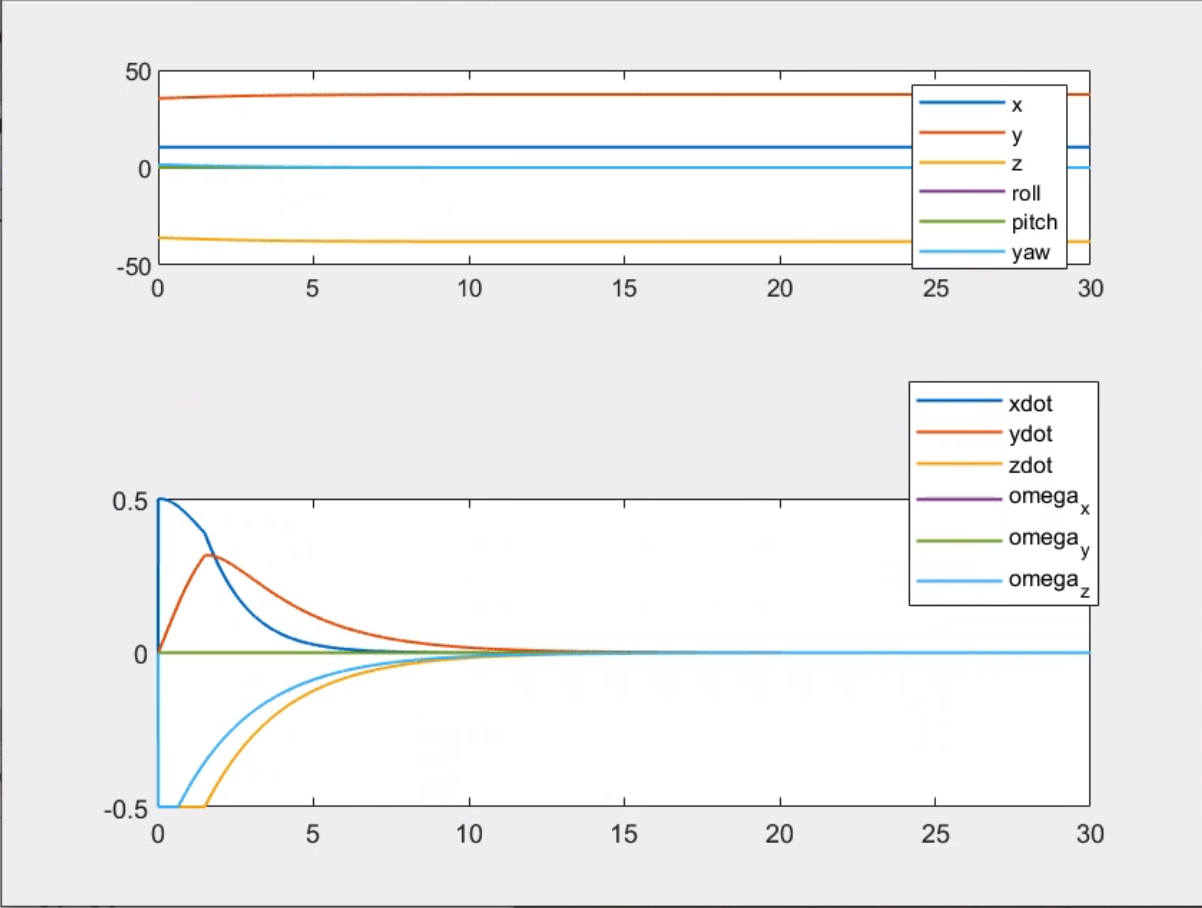
\includegraphics[scale=0.5]{111_ppdot.png}
    \caption{Resulted Graph for the first task}
    \label{graph_1_1}
\end{figure}

\subsubsection{Q2: What is the behaviour if the Horizontal Attitude is enabled or not? Try changing the initial or target orientation in terms of roll and pitch angles. Discuss the behaviour.} 
By default the Horizontal Attitude is enable and has higher priority than the vehicle position task. This results in the UVMS trying to keep a horizontal orientation with respect to the sea floor (Figure  \ref{fig:hae}): if the target position has pitch and roll different from zero, the robot doesn’t perform the vertical position shown in (Figure  \ref{fig:hane}).
When the horizontal attitude is not enabled, the UVMS trying to find the alignment between its frame and the goal one, without taking (of course) into account to stay in parallel with the seafloor. If the target position has pitch or roll, the robot will try to perform them.

%%%%%%% near images %%%%%%% 
\begin{figure}[htp]
\centering
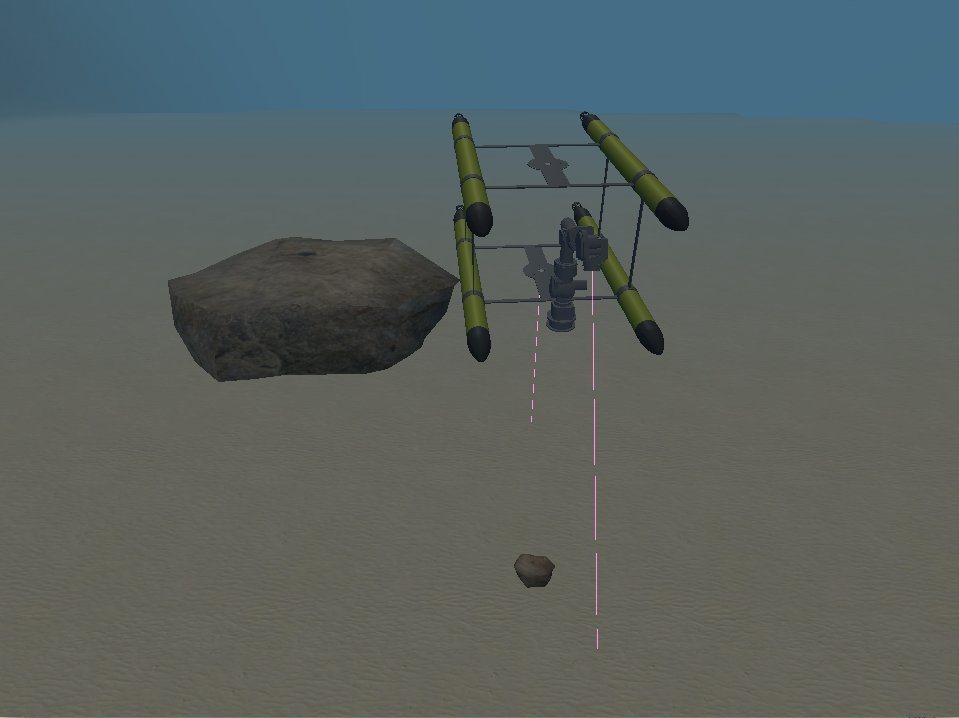
\includegraphics[width=.6\textwidth]{112_HAenabled.png}\caption{Image of the SIM, Horizontal attitude enable, Robot is parallel with the seafloor}
\label{fig:hae}
\centering
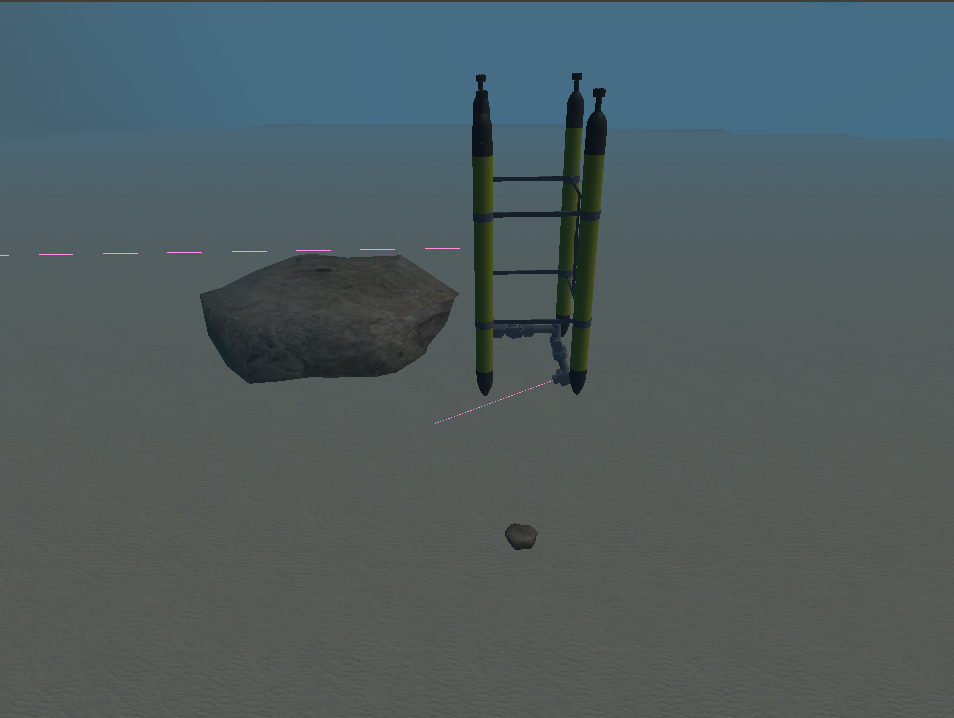
\includegraphics[width=.6\textwidth]{112_HANotenabled.png}\caption{Image of the SIM, Horizontal Attitude not enable, Robot is no more parallel with the seafloor}
\label{fig:hane}
\end{figure}
%%%%%%% %%%%%%%%%% %%%%%%% 

\subsubsection{Q3: Swap the priorities between Horizontal Attitude and the Vehicle Position control task. Discuss the behaviour.}
The problem is the same as before. This time with the priorities switched, if the target, again, as roll or pitch, the robot will try to achieve this orientation. 
So, if we switched the position we will have the same performance as if we disable the Horizontal Attitude task.\\
In the end, it's not usefull to switch the position and it's wrong because the Horizontal Attitude is a Safety Task, so it's, every time, more important (so high priority)than a AD task. 

\subsubsection{Q4: What is the behaviour if the Tool Position control task is active and what if it is disabled? Which of the settings should be used for a Safe Waypoint Navigation action?}
If the Tool Position Control task is enable, the vehicle could not reach the desidered position. If it's enable ad it as higher priority than the Vehicle Position Control task, the robot try to achieve the goal position for the arm, not the ones referred to the vehicle it self. \\
For this reason we split the goal position in two different, the first for the body of the vehicle and another one for the tool. For this particular exercise we didn't use a arm goal position. \\
However, we continue to use the Manipulability task, in order to maintain a safe position for the arm. % HA SENSO PARLARNE QUI?

\clearpage

\subsection{Adding a safety minimum altitude control objective}
Initialize the vehicle at the position:
\begin{displaymath}
\begin{bmatrix} 48.5 & 11.5 & -33 & 0 & 0 &-\pi/2\end{bmatrix}^\top
\end{displaymath} 
Choose as target point for the vehicle position the following one:
\begin{displaymath}
\begin{bmatrix} 50 & -12.5 & -33 & 0 & 0 &-\pi/2 \end{bmatrix}^\top
\end{displaymath}

Goal: Implement a task to control the altitude from the seafloor. Check that at all times the minimum distance from the seafloor is guaranteed.

\subsubsection{Q1: Report the hierarchy of task used and their priorities. Comment how you choose the priority level for the minimum altitude.}
The new hierarchy of tasks is:
\begin{itemize}
	\item Minimum altitude
	\item Manipulability
	\item Horizontal attitude
	\item Vehicle position
\end{itemize}
The news task implemented: \\
Minimum Altitude [R,I,S], it has high priority because it's a safety task, UVM must avoid crashes with the seafloor.

\subsubsection{Q2: What is the Jacobian relationship for the Minimum Altitude control task? How was the task reference computed?}
We need to control the movement along the $z$ axis, so we use the same Jacobian of the vehicle position, but selecting only the component related to the $z$ axis.

%%%%%%% Jacobian Matrix %%%%%%% 
\begin{equation}
\boldsymbol{J}_{mav}=\begin{bmatrix} 0 & 0 & 0 & 0 & 0 & 1
\end{bmatrix}
    \begin{bmatrix}
     & \underset{3\times 3}{\boldsymbol{0}} & \underset{ 3\times 3}{^{w}\boldsymbol{R}_{v}} \\
     \underset{ 6\times 7}{\boldsymbol{0}} \\
     & \underset{ 3\times 3}{^{w}\boldsymbol{R}_{v}} & \underset{3\times 3}{\boldsymbol{0}} \\
    \end{bmatrix}
\end{equation}
%%%%%%% %%%%%%% %%%%%%% %%%%%%% 

Note that in order to select the desired component we used the vector [0 0 0 0 0 1] because the control variable uses a the convention [R P Y X Y Z].
\\
We compute the \textbf{task reference} as the difference between the minimum distance given from the operator and the measured distance vector projected on the world frame:
\begin{equation}
    ^{w}\dot{\overline{\boldsymbol{x}}}_{mav} = k((d_{limit}+\Delta)- ^w d_{sensor})) %delta
\end{equation}
\begin{itemize}
    \item $k$ is the control gain.
    \item $d_{limit}$ is the desired minimum distance from the seafloor.
    \item $ \Delta $ is the safety distance at which the activation of the task triggers.
    \item $^w d_{sensor}$ is the distance vector measured by the sensor and projected on the world frame.
\end{itemize} 

\begin{figure}[t]
    \centering
    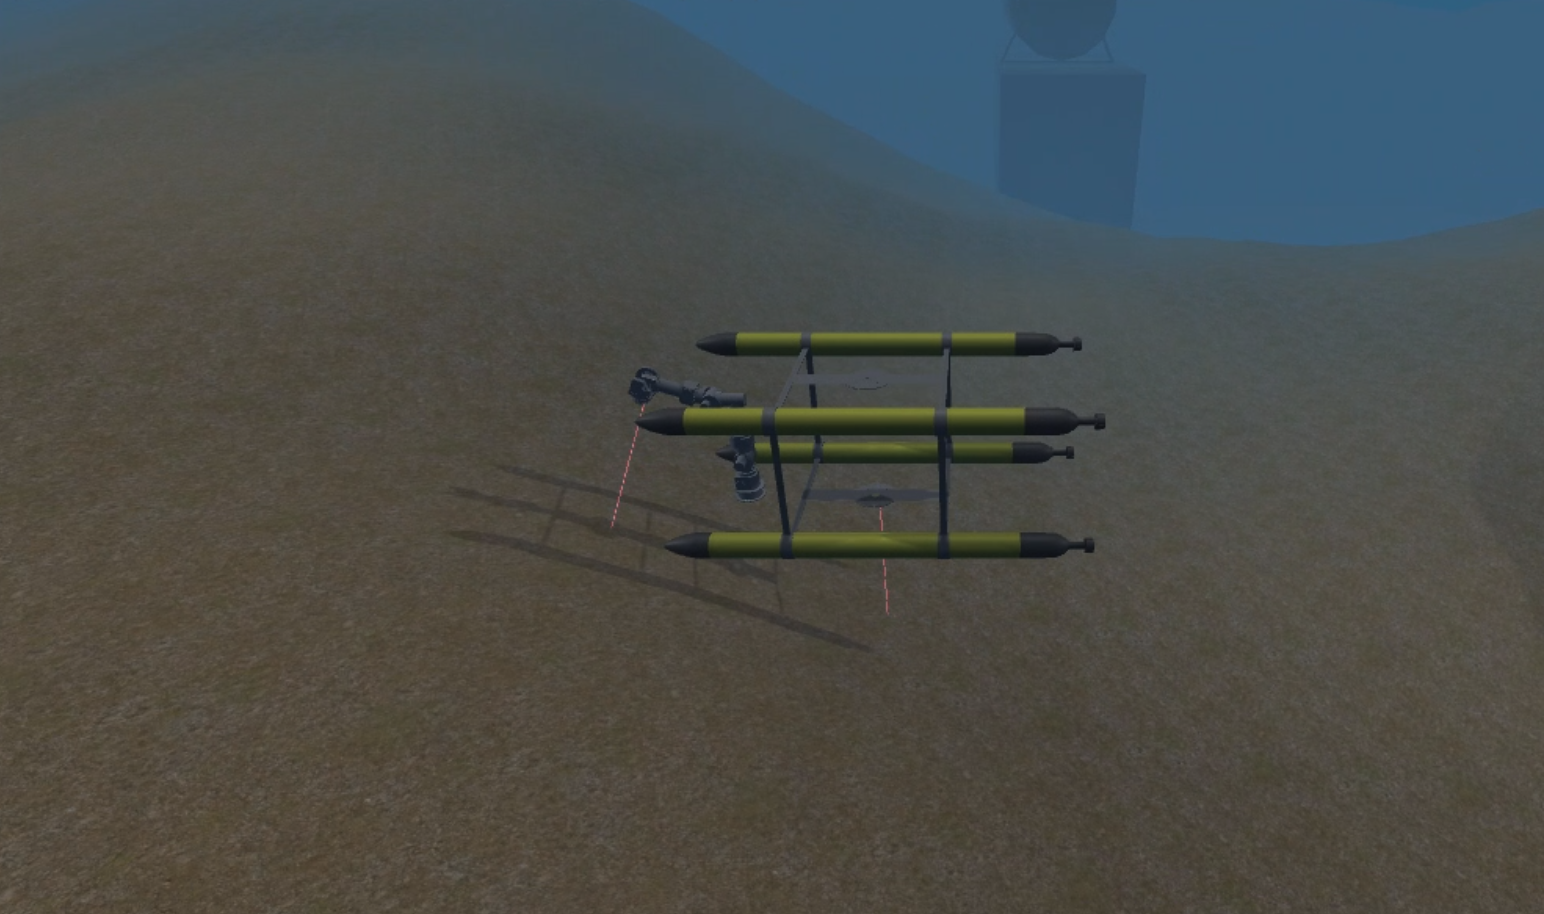
\includegraphics[scale=0.4]{122_MAV1m.png}
    \caption{Image of the SIM, Minimum Altitude Vehicle set to 0.5m, Robot is following the seafloor}
    \label{images_2_1}
\end{figure}

%Gray box for defining code implemented or referred to
\colorbox{mygray}{\parbox{0.9\textwidth}{Code for Exercise: \\
\texttt{Compute Task Reference -> MAV Control}\\
}}

\subsubsection{Q3: Try imposing a minimum altitude of 1, 5, 10 m respectively. What is the behaviour?}
To achieve this task we perform the different minimum altitude, all with the same $k$ gain (equal to $0.2$), and the same $\Delta$ for the inequality nature of the problem (equal to $0.5 m$).

\begin{itemize}
    \item \textbf{10 m:} It seems no a reasonable value. The UVMS has initial position below this threshold, so it start floating to the surface very quickly (it is possible to notice this huge vertical velocity in the graph (Figure \ref{10m_ppdot}), $\dot{z}$). Of course, the task is not accomplished because the target position is far from the threshold.
    \item \textbf{5 m:} The same as before, the activation is active at the first instant because again the initial position is below the minimum altitude. This control task is a safety one, so every time the UVMS is under the minimum altitude is active and it has the highest priority. Again, it seems no reasonable to perform such big gap with the seafloor (Reported graph, Figure \ref{5m_ppdot}).
    \item \textbf{1 m:} This time the problem is the opposite. The control task is no more active at the starting instant. The UVMS starts to accomplish the Vehicle Position Control task, when the seafloor present an hill the UVMS start to follow the pattern (Figure \ref{1m_ppdot}). However, there are some troubles during the navigation because the "noise" of the robot, with only 1 meter of distance (and no $\Delta$ that could prevent this), could touch the soil because the sensor it's on the center of the vehicle.
\end{itemize}

\subsubsection{Q4: How was the sensor distance processed?}
 
 ${^{v}d_{sensor}}$ is the distance vector measured by the sensor, so we need to projected it on the world frame, to do this we apply a rotation:
 
 %ESPRESSIONE DEL MOTHERFUCKER SENSOR DISTANCE ON THE WORLD FRAME
 \begin{equation}
     {^{w}\boldsymbol{d}_{sensor}} = {^{w}\boldsymbol{R}_{v}} {^{v}\boldsymbol{d}_{sensor}}
 \end{equation}
 
 Again we are only interested on the $z$ axis. The $\boldsymbol{d}_{sensor}$ are the vectors build as:
 $\begin{bmatrix}0 & 0 & d_{seafloor} \end{bmatrix}^\top$
\\

 %Gray box for defining code implemented or referred to
\colorbox{mygray}{\parbox{0.9\textwidth}{Code for Exercise: \\
\texttt{TO DO}\\
\texttt{TO DO}
}}

%%%%%%%% MINI PAGE IMAGES 10 m %%%%%%%%
\begin{figure}[htpb] 
\begin{minipage}{0.40\textwidth}  
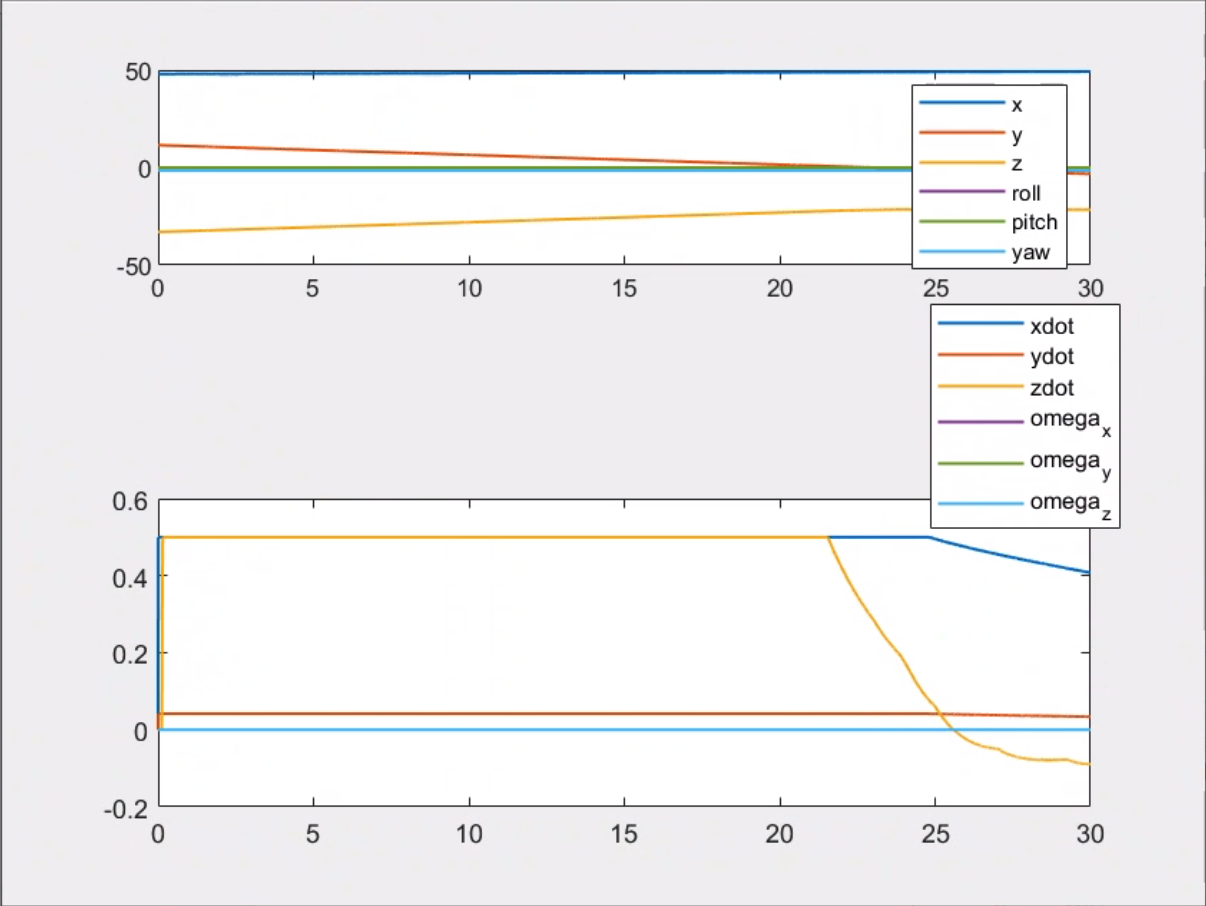
\includegraphics[width=\textwidth]{123_10m_ppdot.png}
\caption{Position and velocities during the Minimum Altitude Vehicle task imposed 10m threshold}\label{10m_ppdot} 
\end{minipage}  
\hspace{0.2\textwidth} 
\begin{minipage}{0.43\textwidth}  
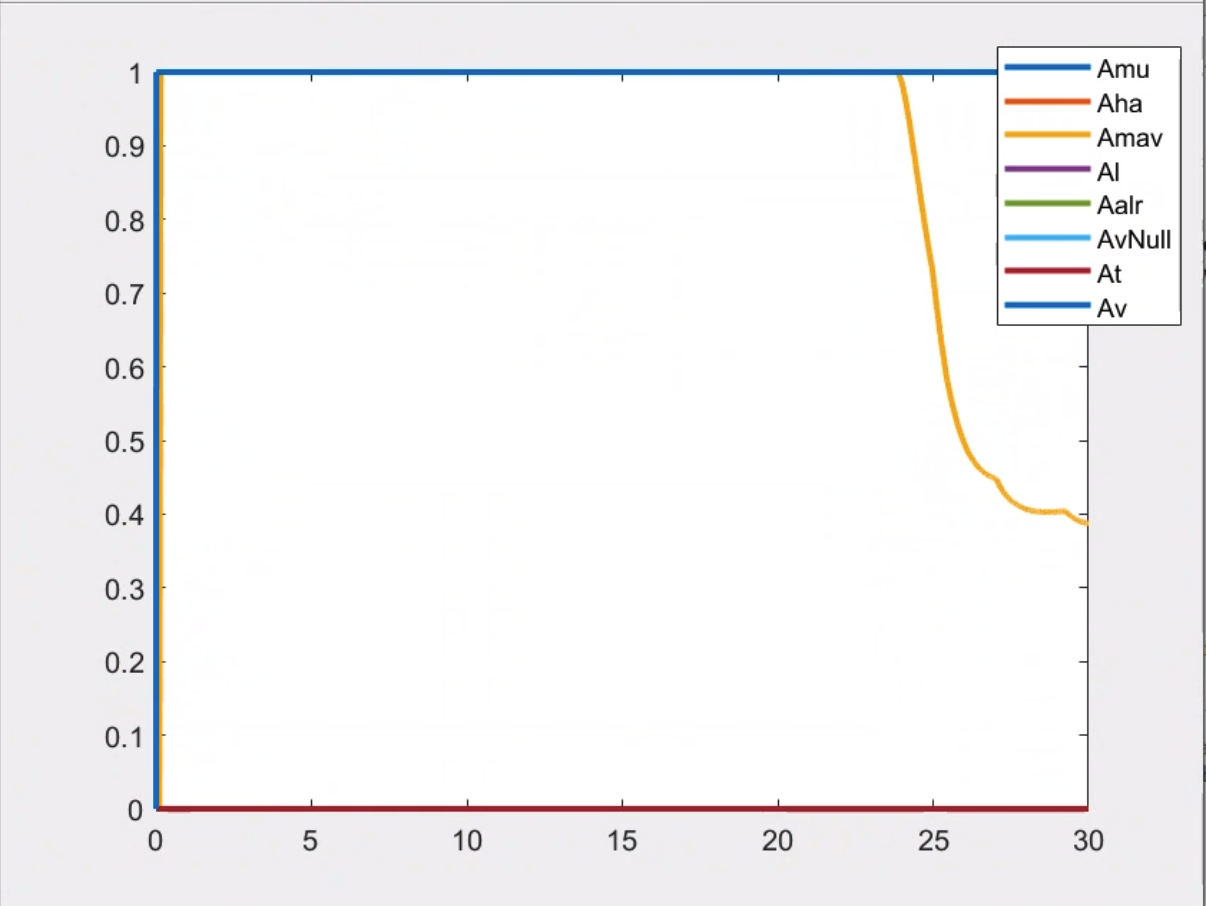
\includegraphics[width=\textwidth]{123_10m_A.png}
\caption{Positions and Velocity with medium}\label{10m_A} 
\end{minipage} 
\end{figure}
%%%%%%%% MINI PAGE IMAGES %%%%%%%%

%%%%%%%% MINI PAGE IMAGES 5 m %%%%%%%%
\begin{figure}[htpb] 
\begin{minipage}{0.40\textwidth}  
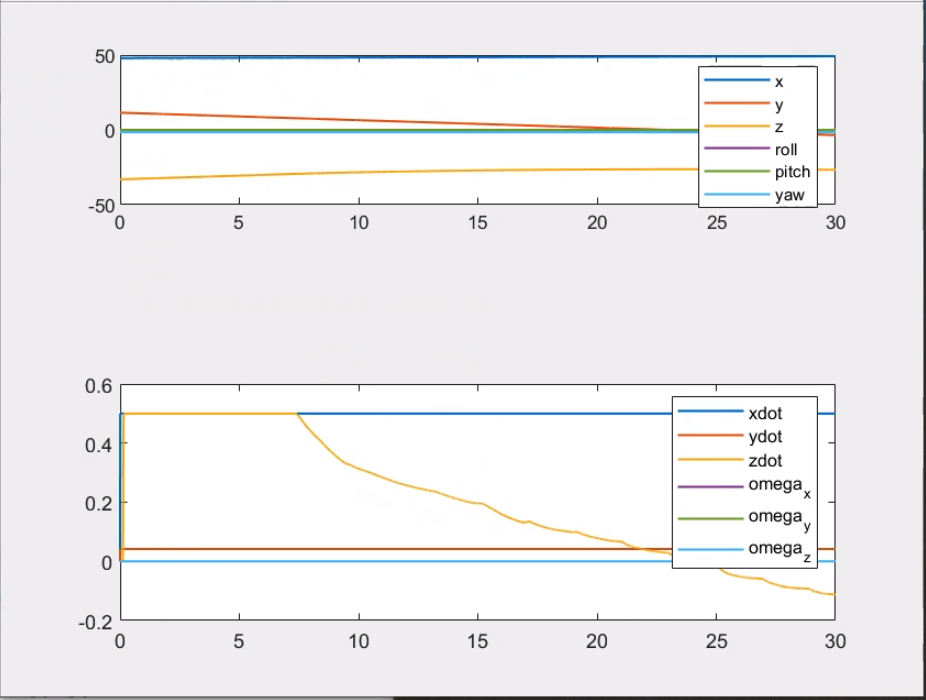
\includegraphics[width=\textwidth]{123_5m_ppdot.png}
\caption{Position and velocities during the Minimum Altitude Vehicle task imposed 10m threshold}\label{5m_ppdot} 
\end{minipage}  
\hspace{0.2\textwidth} 
\begin{minipage}{0.43\textwidth}  
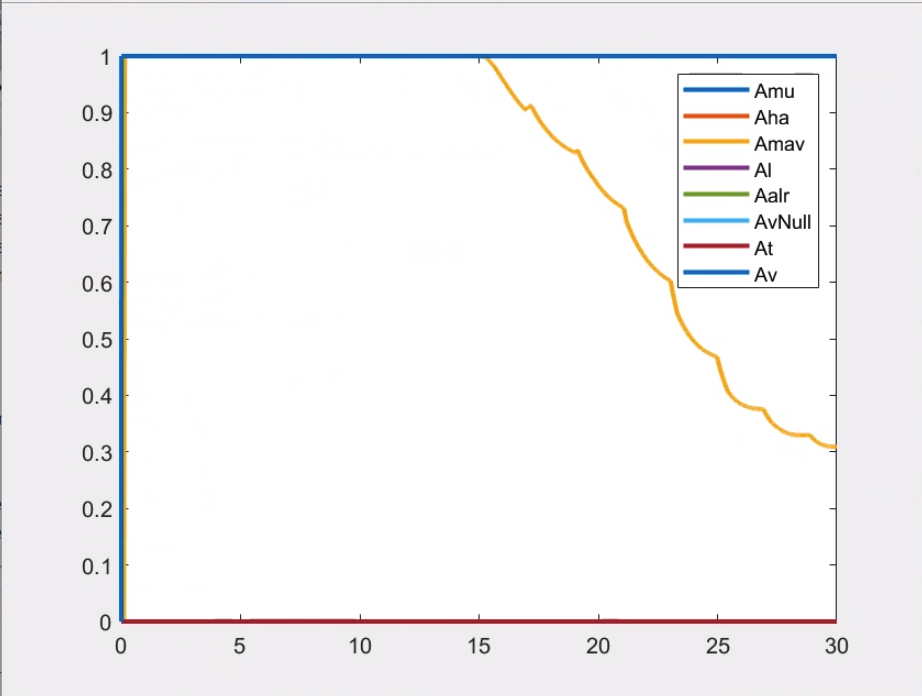
\includegraphics[width=\textwidth]{123_5m_A.png}
\caption{Positions and Velocity with medium}\label{5m_A} 
\end{minipage} 
\end{figure}
%%%%%%%% MINI PAGE IMAGES %%%%%%%%

%%%%%%%% MINI PAGE IMAGES 1 m %%%%%%%%
\begin{figure}[htpb] 
\begin{minipage}{0.40\textwidth}  
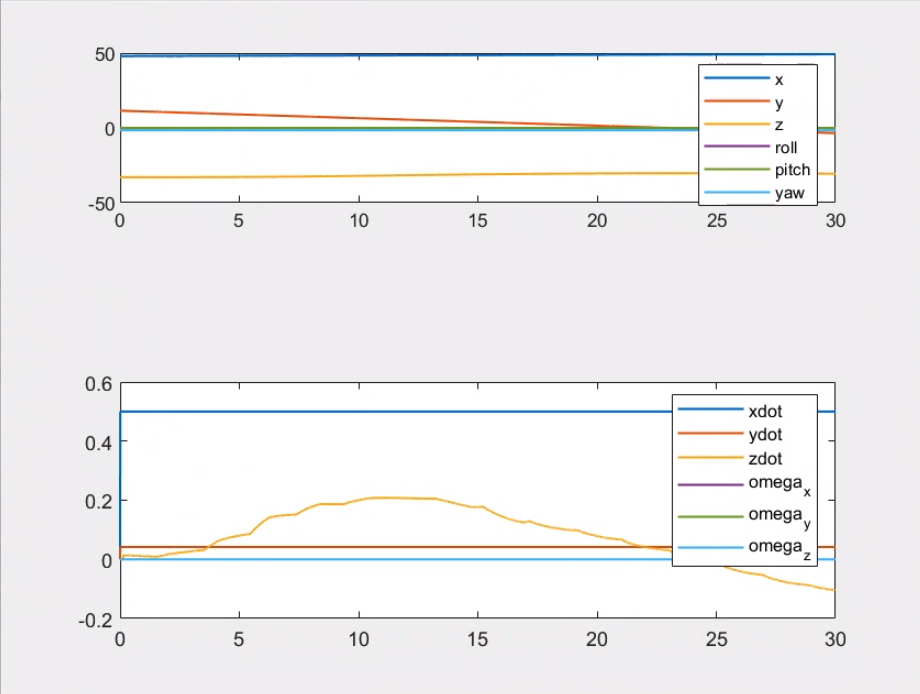
\includegraphics[width=\textwidth]{123_1m_ppdot.png}
\caption{Position and velocities during the Minimum Altitude Vehicle task imposed 1m threshold}\label{1m_ppdot} 
\end{minipage}  
\hspace{0.2\textwidth} 
\begin{minipage}{0.40\textwidth}  
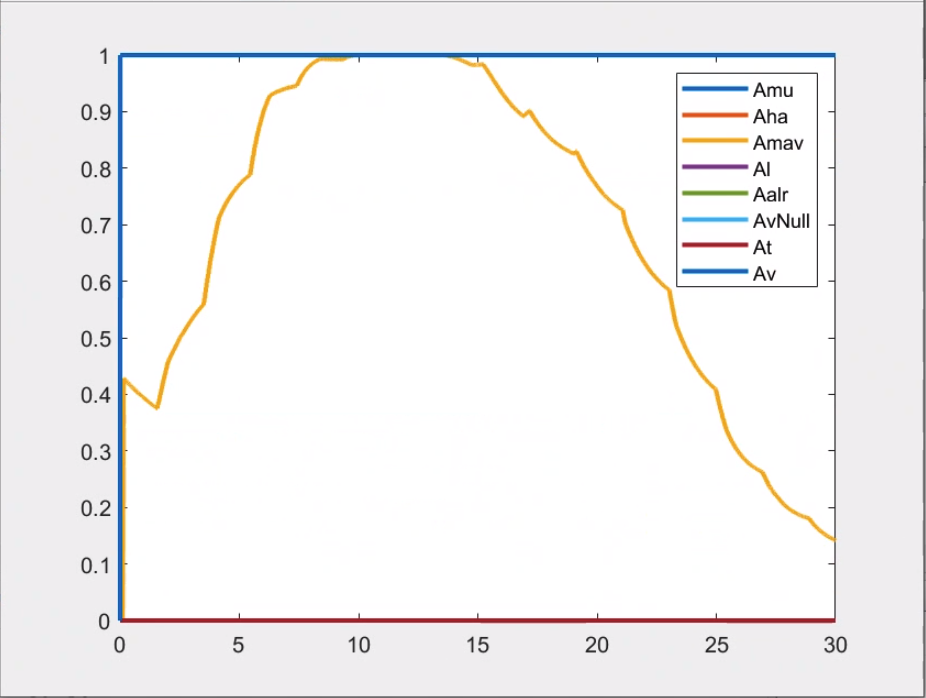
\includegraphics[width=\textwidth]{123_1m_A.png}
\caption{Positions and Velocity with medium}\label{1m_A} 
\end{minipage} 
\end{figure}
%%%%%%%% MINI PAGE IMAGES %%%%%%%%

\clearpage

\section{Exercise 2: Implement a Basic “Landing” Action.}
\subsection{Adding an altitude control objective}
Initialize the vehicle at the position:
\begin{displaymath}
\begin{bmatrix} 10.5 & 37.5 & -38 & 0 & -0.06 & 0.5 \end{bmatrix}^\top
\end{displaymath} 

Goal: add a control task to regulate the altitude to zero.

\subsubsection{Q1: Report the hierarchy of task used and their priorities. Comment how you choose the priority level for the altitude control task.}
The new hierarchy of tasks is:
\begin{enumerate}
	\item Manipulability
	\item Horizontal attitude
	\item Landing
\end{enumerate}
\begin{description}
\item \textbf{Landing} [R, E, AD], is the new task. It is a Action Defining task, so it has the same priority as the Vehicle position task.
\end{description}
The task Minimum Altitude is not enable now, because (of course) we need, only, to land.

\begin{figure}[h]
    \centering
    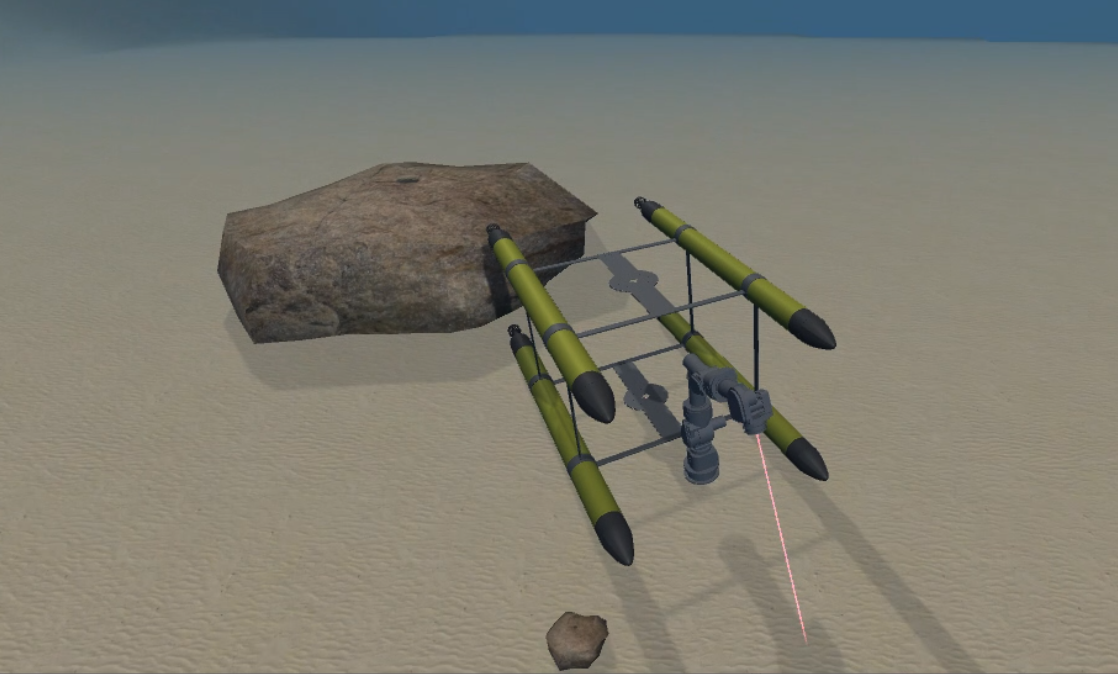
\includegraphics[scale=0.4]{211_Landing.png}
    \caption{Implemented basic "Landing" action}
    \label{images_2_3_1}
\end{figure}

\subsubsection{Q2: What is the Jacobian relationship for the Altitude control task? How was the task reference computed?}

\begin{equation}
\boldsymbol{J}_{land}=\begin{bmatrix} 0 & 0 & 0 & 0 & 0 & 1
\end{bmatrix}
    \begin{bmatrix}
     & \underset{3\times 3}{\boldsymbol{0}} & \underset{ 3\times 3}{^{w}\boldsymbol{R}_{v}} \\
     \underset{6\times 7}{\boldsymbol{0}} \\
     & \underset{ 3\times 3}{^{w}\boldsymbol{R}_{v}} & \underset{3\times 3}{\boldsymbol{0}} \\
    \end{bmatrix}
\end{equation}
As before the Jacobian take into account only the z component (using the pre-multiplication with the [0 0 0 0 0 1] matrix). 
\\
We compute the \textbf{task reference} as as the difference between the seafloor and the measured distance projected on the world frame:

\begin{equation}
    ^{w}\dot{\overline{\boldsymbol{x}}}_{land} = k((seafloor + safeguard) - ^w d_{sensor})) %delta
\end{equation}
\begin{itemize}
    \item $k$ is the control gain.
    \item $seafloor$ is simply 0.
    \item $safeguard$ is set to 0.15m  to avoid interpenetration between UVMS and the seafloor.
    \item $^w d_{sensor}$ is the distance vector measured by the sensor and projected on the world frame.
\end{itemize} 

%Gray box for defining code implemented or referred to
\colorbox{mygray}{\parbox{0.9\textwidth}{Code for Exercise: \\
\texttt{TO DO}\\
\texttt{TO DO}
}}

\subsubsection{Q3: how does this task differs from a minimum altitude control task?}
There are two major difference, the first one is that this task it isn't a safety task, it's a Action-Defining task. The Minimum Altitude it's used to avoid crash with the seafloor, the Landing task it's like the Vehicle Position task, and, as this one, it has low priority.
The second big difference is that the Minimum altitude is an Inequality task rather than the Landing that is and equality. For this reason, as visible on the graphs below (Figure \ref{213}), MAV is active when we are under the imposed threshold, Landing is active only when is called and stay active until we touch the seafloor.


%%%%%%%% MINI PAGE IMAGES %%%%%%%%
\begin{figure}[!h]
    \centering
    \begin{minipage}{0.50\textwidth}
    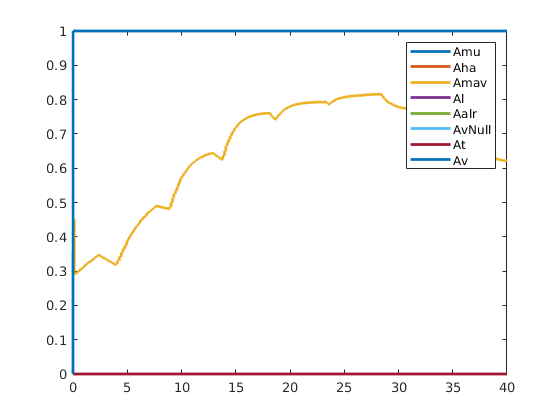
\includegraphics[scale=0.5]{213_MAV_A.png}
    \caption{Graph MAV}
    \label{213}
    \end{minipage}
\hfill
    \centering
    \begin{minipage}{0.50\textwidth}
    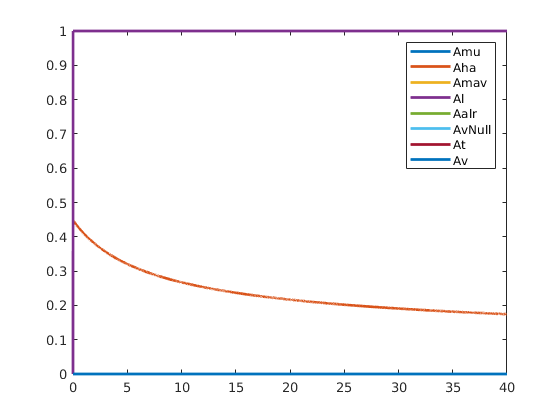
\includegraphics[scale=0.5]{213_Landing_A.png}
    \caption{Graph Landing}
    \end{minipage}
\end{figure}
%%%%%%%% MINI PAGE IMAGES %%%%%%%%

\clearpage

\subsection{Adding mission phases and change of action}
Initialize the vehicle at the position:
\begin{displaymath}
\begin{bmatrix} 8.5 & 38.5 & -36 & 0 & -0.06 & 0.5 \end{bmatrix}^\top
\end{displaymath} 
Use a "safe waypoint navigation action" to reach the following position: 
\begin{displaymath}
\begin{bmatrix} 10.5 & 37.5 & -38 & 0 & -0.06 & 0.5 \end{bmatrix}^\top
\end{displaymath} 
When the position has been reached, land on the seafloor using the basic "landing" action.

\subsubsection{Q1: Report the unified hierarchy of tasks used and their priorities.}

We have two different actions, with this hierarchy and activations: 
%%%%%% TABLE %%%%%%%%%
\begin{center}
\begin{tabular}{ | c | c | c | c |}
\hline
 Control Task & \texttt{Code name} & Action A & Action B \\
\hline
 Minimum Altitude Vehicle &  \texttt{mav} & Active & Inactive  \\  
 Manipulabity &  \texttt{mu} & Active & Active  \\
 Horizontal Attitude &  \texttt{ha} & Active & Active \\
 Landing & \texttt{l} &Inactive & Active \\
 Vehicle Position &  \texttt{v} &Active & Inactive \\
 \hline
\end{tabular}
\end{center}

\begin{description}
\item Action A, perform the safe waypoint navigation. All the safety task are enable. 
\item Action B, the robot need simply to land, it just performs the previous exercise task, of course, we need to inactivate the Minimum Altitude.
\end{description}
 
%%%%%% TABLE %%%%%%%%%


%Gray box for defining code implemented or referred to
\colorbox{mygray}
{\parbox{0.9\textwidth}{Code for Exercise: \\
\texttt{ComputeMissionPhase}\\
}}

\subsubsection{Q2: How did you implement the transition from one action to the other?}
From Action A to Action B, we compute the cartesian error between the goal position and the actual. When the error is below our threshold (0.15m) the mission phase changes. 

When we want to Inactivate a running task, we perform a Decreasing Bell Shape function in order to perform a smooth transition (like Minimum Altitude and Vehicle Position task, both Inactivated in the same method). In the same way, we also perform an Increasing Bell Shape function to perform a smooth activation of the Landing task. We perform the bell shaped function based on the mission phase time, this help us to fix the time when we switch from an Action to the other one, and perform shape from 0 to 0.2 seconds, to avoid spike to the motors.
\begin{figure}[!htb]
    \centering
    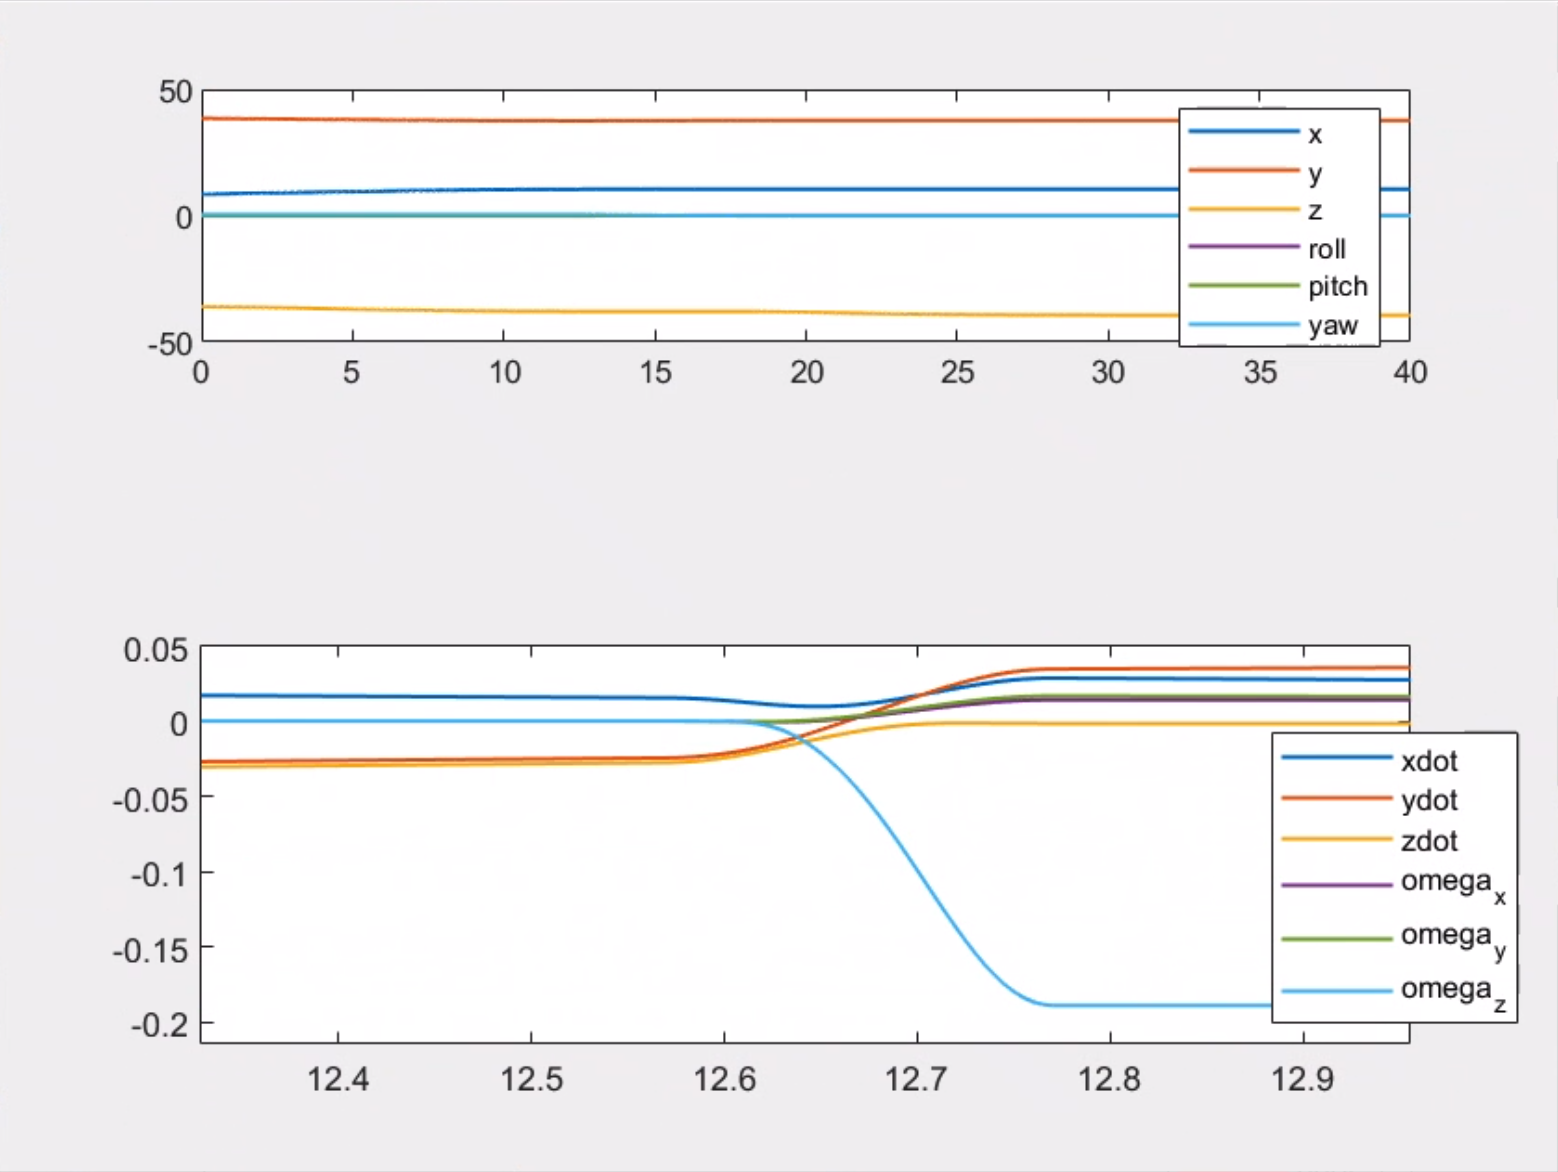
\includegraphics[scale=0.25]{222_smooth_ppdot.png}
    \caption{Zoom of the smooth change}
    \label{images_2_3_1}
\end{figure}

We found this more adeguate that the previous attempt, in which we performed the shape based on the error distance.


 
\clearpage

\section{Exercise 3: Improve the “Landing” Action}
\subsection{Adding an alignment to target control objective}
If we use the landing action, there is no guarantee that we land in from of the nodule/rock. We need to add additional constraints to make the vehicle face the nodule. The position of the rock is contained in the variable \texttt{rock\_center}. 

Initialize the vehicle at the position:
\begin{displaymath}
\begin{bmatrix} 8.5 & 38.5 & -36 & 0 & -0.06 & 0.5 \end{bmatrix}^\top
\end{displaymath} 
Use a "safe waypoint navigation action" to reach the following position: 
\begin{displaymath}
\begin{bmatrix} 10.5 & 37.5 & -38 & 0 & -0.06 & 0.5 \end{bmatrix}^\top
\end{displaymath} 
Then land, aligning to the nodule.

Goal: Add an alignment task between the longitudinal axis of the vehicle ($x$ axis) and the nodule target. In particular, the $x$ axis of the vehicle should align to the projection, on the inertial horizontal plane, of the unit vector joining the vehicle frame to the nodule frame.

\subsubsection{Q1: Report the unified hierarchy of tasks used and their priorities. Comment the behaviour.}
We have three different actions, with this hierarchy and activations:
%%%%%% TABLE %%%%%%%%%
\begin{center}
\begin{tabular}{ | c | c | c | c | c |}
\hline
 Control Task & \texttt{Code name} & Action A & Action B & Action C\\
 \hline
 Minimum Altitude Vehicle &  \texttt{mav} & Active & Active & Inactive\\  
 Manipulabity &  \texttt{mu} & Active & Active & Active\\
 Horizontal Attitude &  \texttt{ha} & Active & Active & Active\\
 Alignment to the rock & \texttt{alr} & Inactive & Active & Active \\
 Landing & \texttt{l} &Inactive & Inactive & Active \\
 Vehicle Position &  \texttt{v} &Active & Inactive & Inactive\\
 \hline
\end{tabular}
\end{center}
%%%%%% TABLE %%%%%%%%%
\begin{description}
\item \textbf{Alignment to rock} [R, I, P], it is a prerequisite task, so it has higher priority than the Action Defining tasks. Inequality, because we admit an $value$.  \ocio 
\end{description}

\begin{figure}[h]
    \centering
    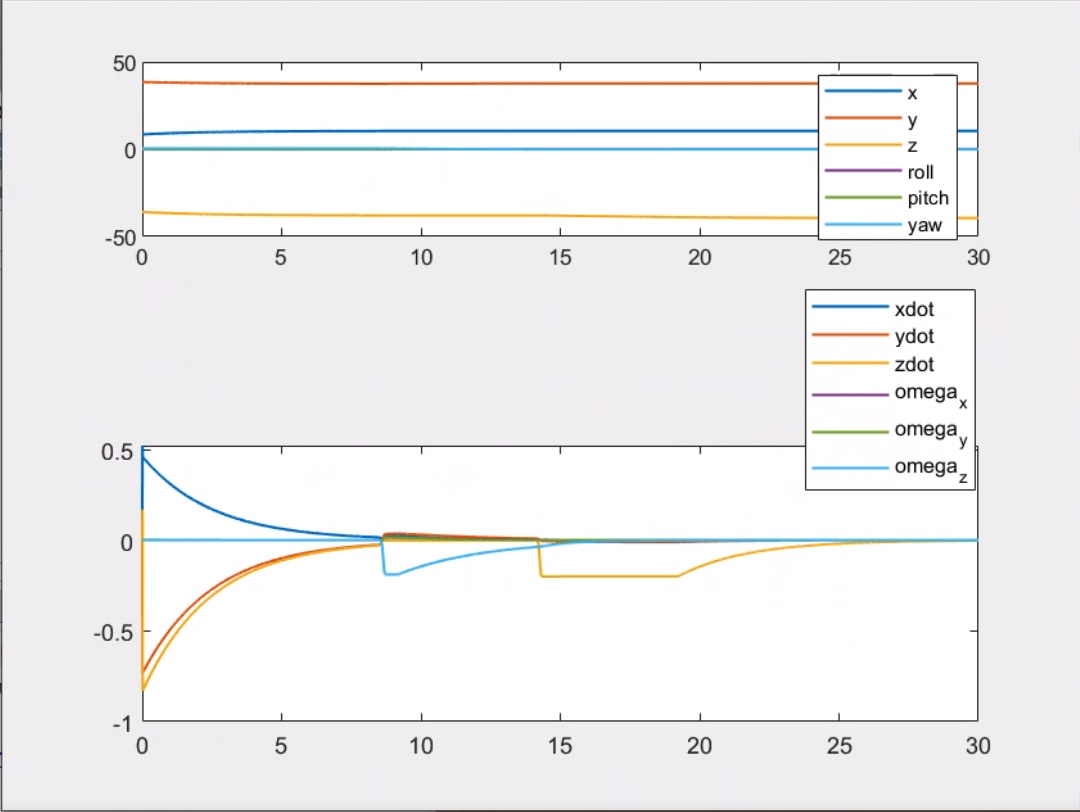
\includegraphics[scale=0.3]{311_ppdot.png}
    \caption{Positions and velocities during the three actions.}
    \label{graphes3}
\end{figure}

\begin{description}
	\item Action A, again, a safe waypoint navigation with all the safety tasks enable (Figure \ref{311a}). 
	\item Action B, it is the action that performs the alignment to the rock, with all the safety task enable (Figure \ref{311b}). 
	\item Action C, alignment to the nodule is not disable because, while the UVMS starts landing, we disable smoothly the alignment. In this case, while the robot is performing the landing, it continue to rotate to optimize the orientation (Figure \ref{311c}).
\end{description}



%%%%%%% near images %%%%%%% 
\begin{figure}[htp]
\centering
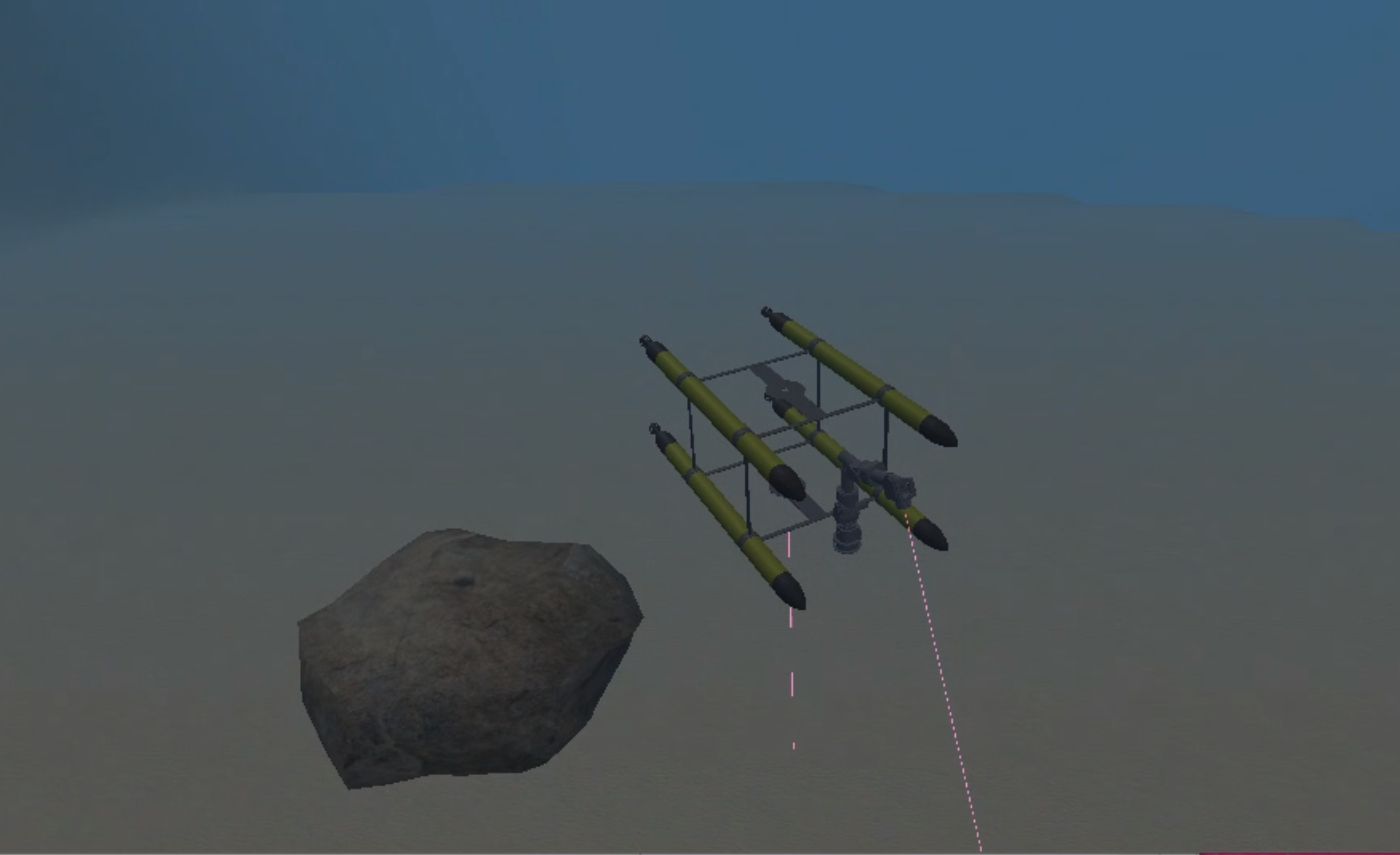
\includegraphics[width=.6\textwidth]{312_Nav.png}\caption{Action A: Navigation till the target position}\label{311a}
\centering
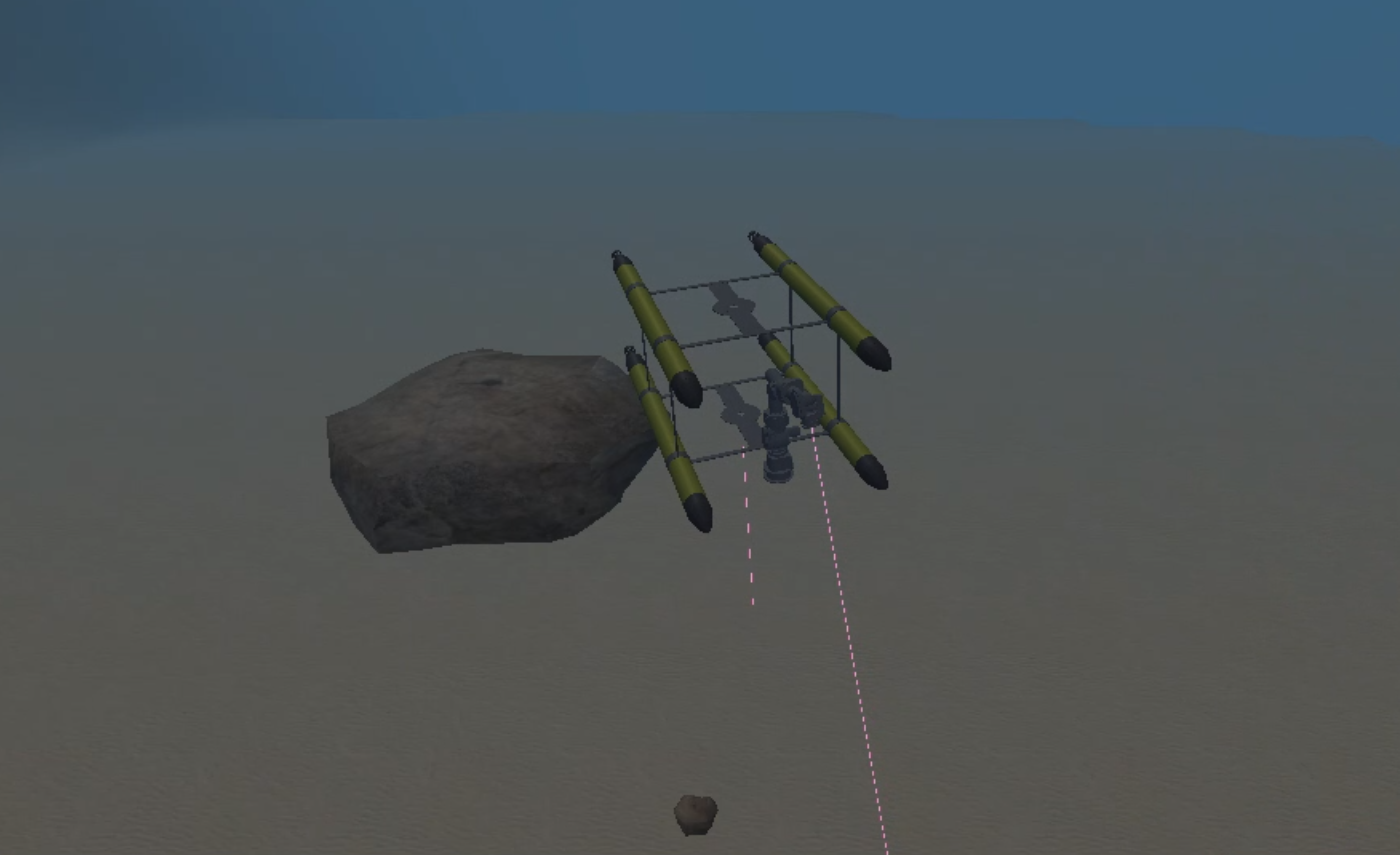
\includegraphics[width=0.6\textwidth]{312_Alr.png}\caption{Action B: Alignment with the rock center}\label{311b}
\centering
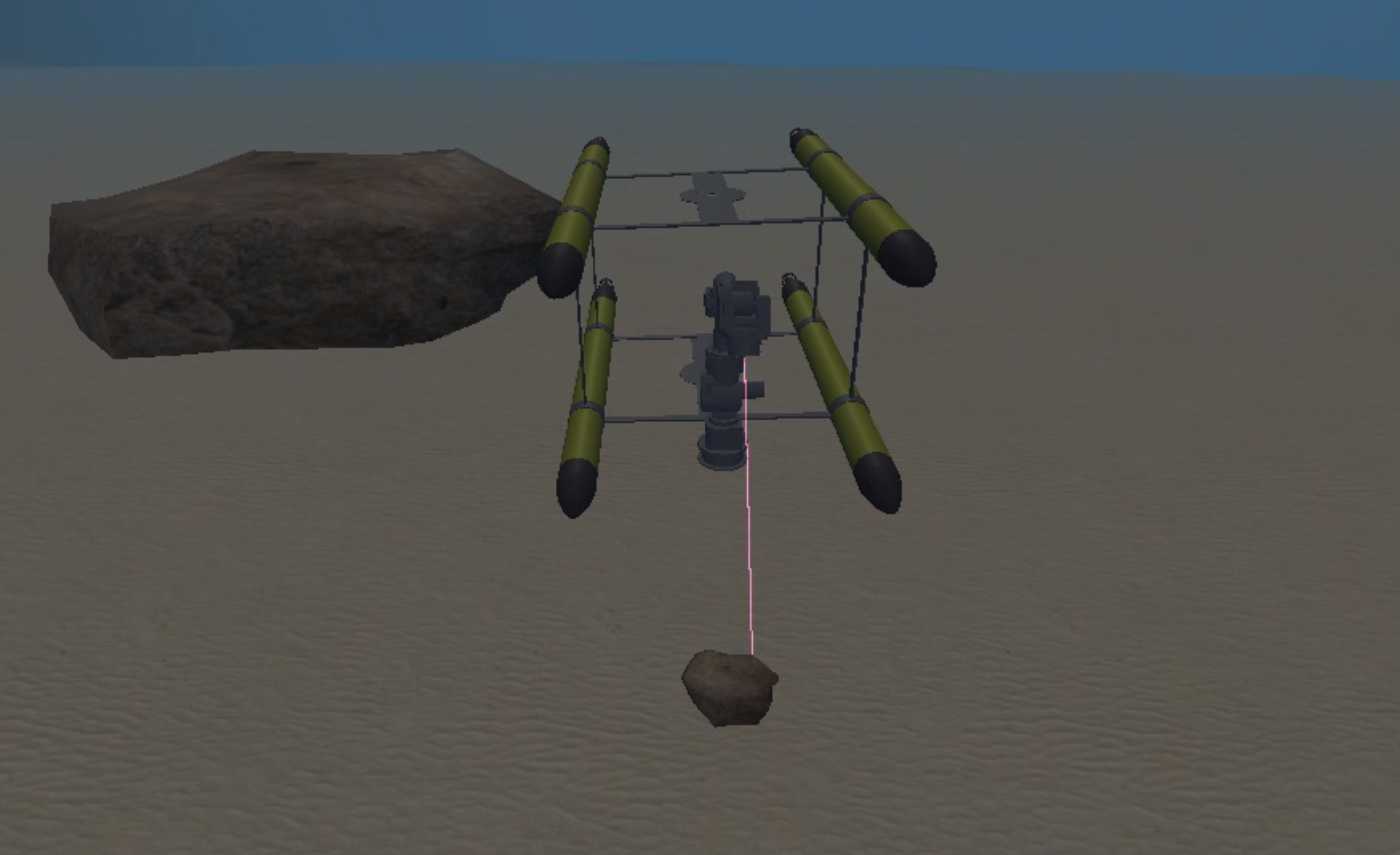
\includegraphics[width=.6\textwidth]{312_Land.png}\caption{Action C: Landing, final action}\label{311c}
\label{fig:missionphase3}
\end{figure}
%%%%%%% %%%%%%%%%% %%%%%%% 
\clearpage

\subsubsection{Q2: What is the Jacobian relationship for the Alignment to Target control task? How was the task reference computed?} \
COPIARE JACOBIANA \ocio

\subsubsection{Q3: Try changing the gain of the alignment task. Try at least three different values, where one is very small. What is the observed behaviour?} \no
We performed tests with different gain values for the task reference:
\begin{itemize}
	\item Very Small = $0,1$
	\item Medium = $0,6$
	\item Big = $1,2$
\end{itemize}
First, looking at the positions and velocities graphs, it is clear that between the medium (Figure \ref{ppdot_w_m}) and the big gain (Figure \ref{ppdot_w_b}) there are no such important differences, it's only clear that with the big gain that transition between the two phases are not so smooth as for the medium one. Of course, the saturation helps the case with the big gain to not perform a too high velocity. 
For the very small gain, the resulted graph is very different (Figure \ref{ppdot_w_s}), because it's clear that the very low velocity performed during the allignment doesn't help to reach the desidered posiiton. In our 30 seconds simulation is impossible for the UVMS to allign correctly. However, also improving the simulation time, it's clear that it is too slow to accomplish our goal.

From the point of view of the activations and the errors, there aren't different results than before. Medium and big gain graphs are very similar (almost identical) and the very small gain graph confirm the previous senteces.
%%%%%%%% MINI PAGE IMAGES %%%%%%%%
\begin{figure}[htpb] 
\begin{minipage}{0.40\textwidth}  
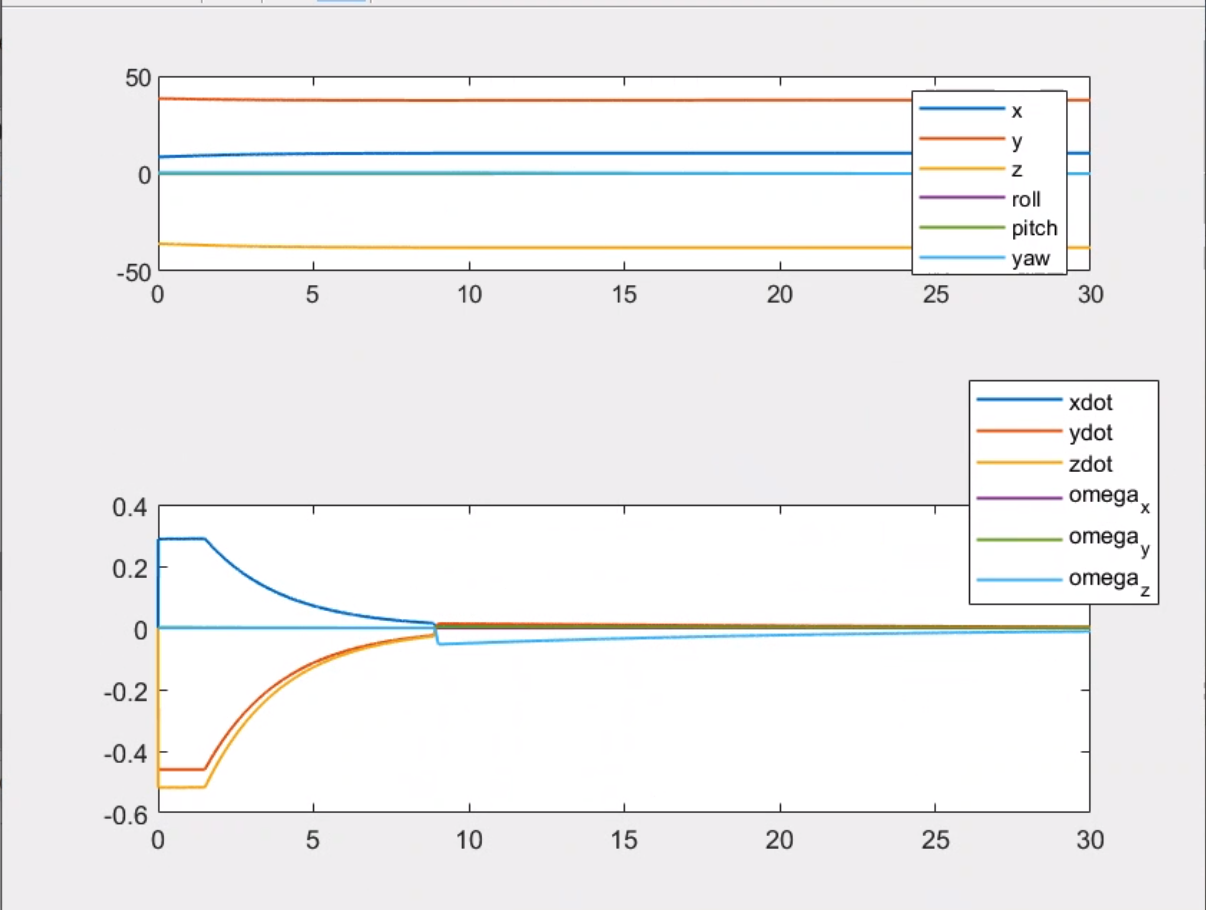
\includegraphics[width=\textwidth]{313_s_ppdot.png}
\caption{Positions and Velocity with small gain}\label{ppdot_w_s} 
\end{minipage}  
\hspace{0.2\textwidth} 
\begin{minipage}{0.40\textwidth}  
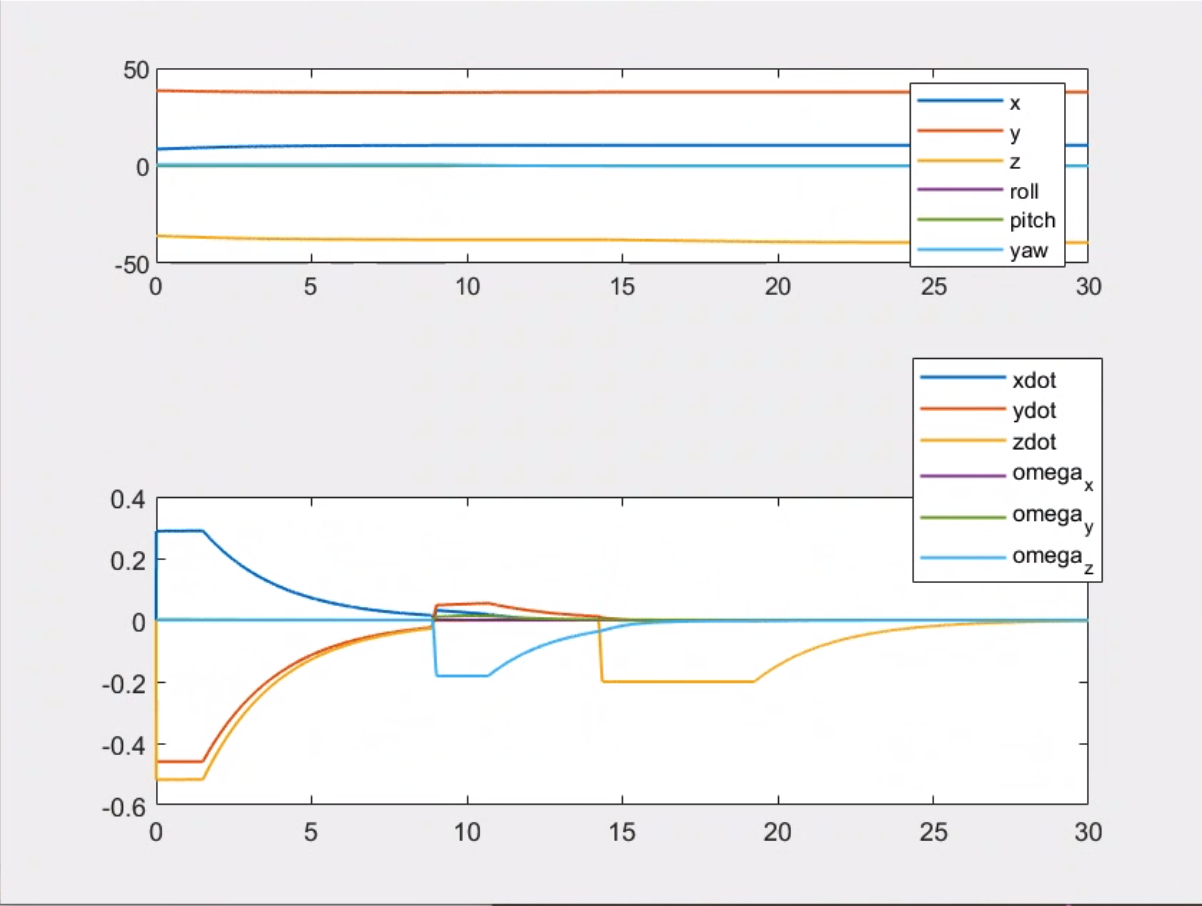
\includegraphics[width=\textwidth]{313_m_ppdot.png}
\caption{Positions and Velocity with medium gain}\label{ppdot_w_m} 
\end{minipage} 
\hspace{0.2\textwidth} 
\begin{minipage}{0.40\textwidth}  
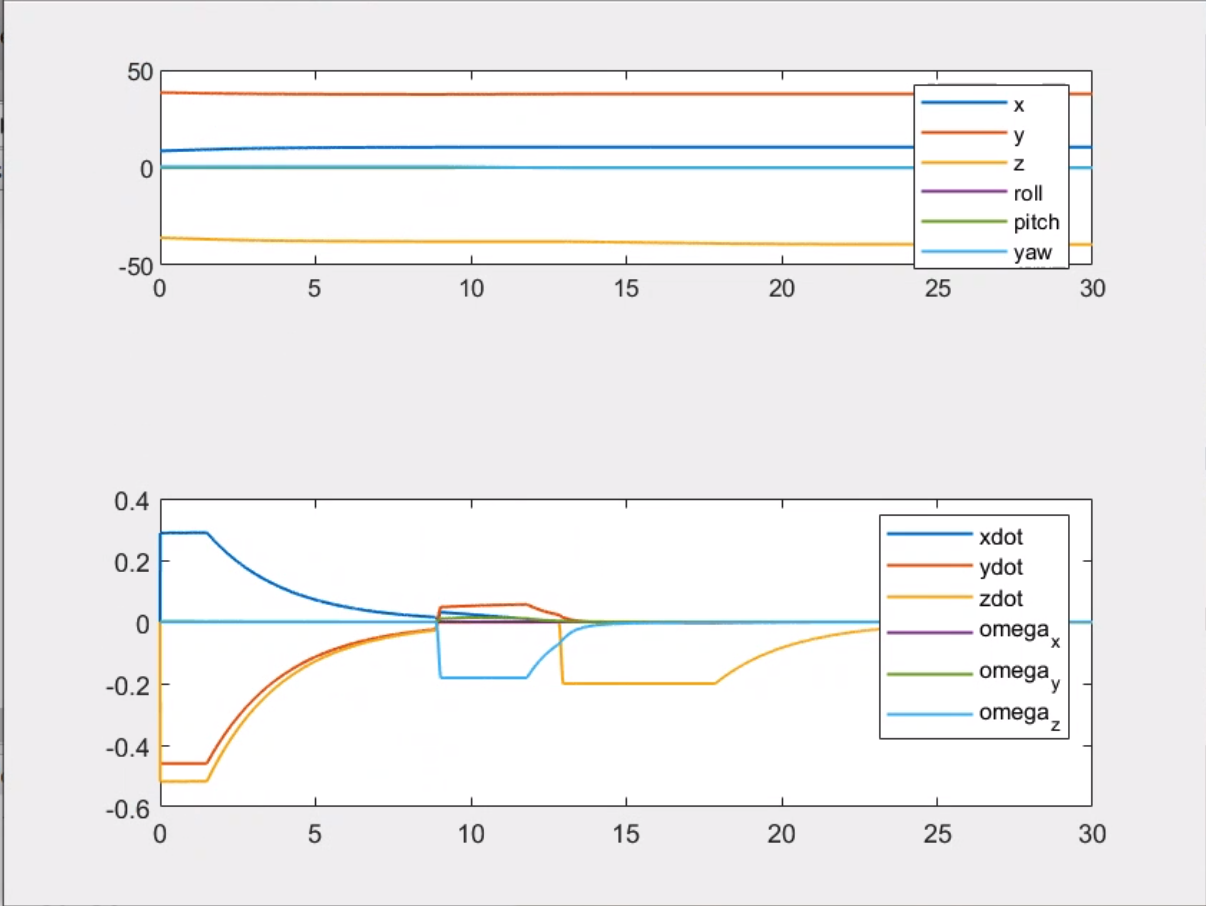
\includegraphics[width=\textwidth]{313_b_ppdot.png}
\caption{Positions and Velocity with big gain}\label{ppdot_w_b} 
\end{minipage}
\end{figure}
%%%%%%%% MINI PAGE IMAGES %%%%%%%%
\begin{figure}[htpb] 
\begin{minipage}{0.40\textwidth}  
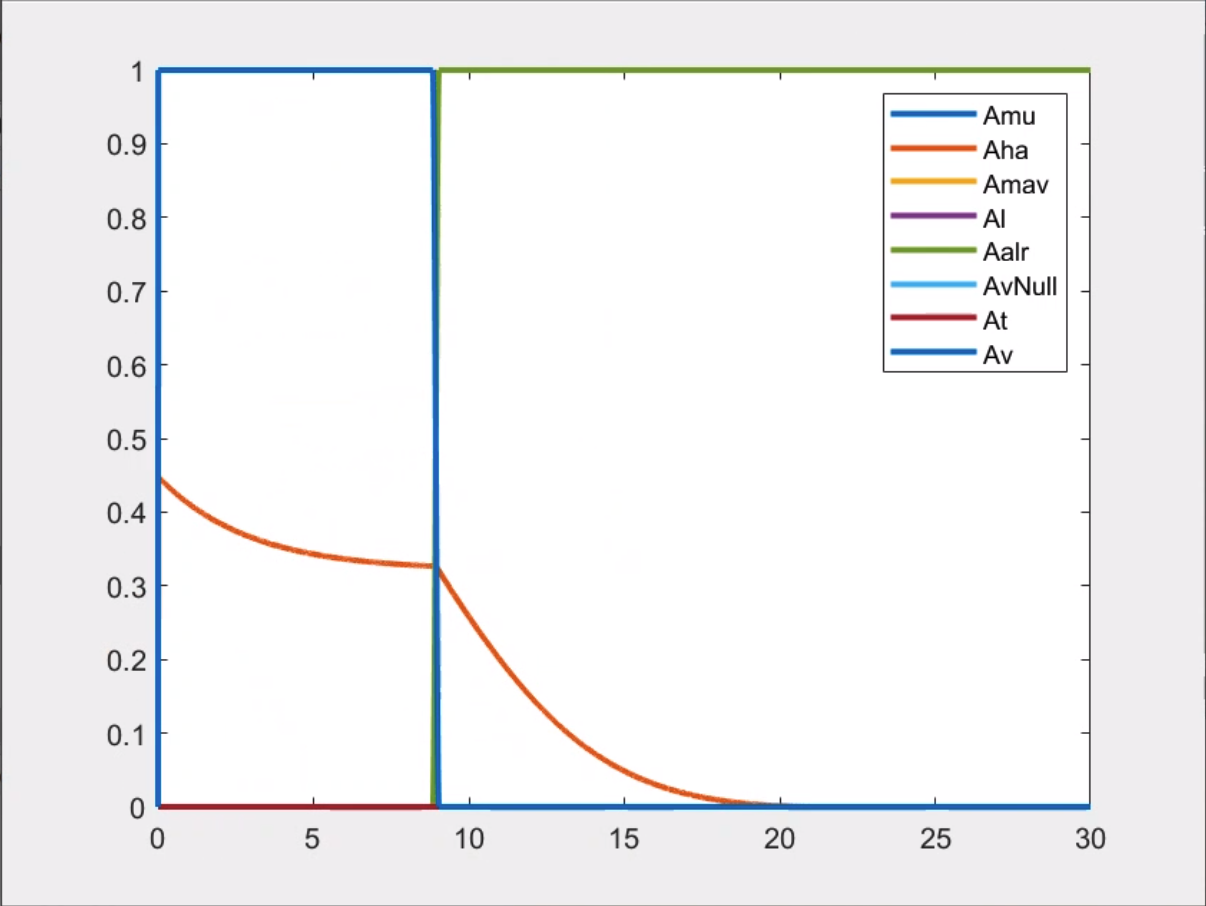
\includegraphics[width=\textwidth]{313_s_Activation.png}
\caption{Activations with very small gain}\label{act_w_s} 
\end{minipage}  
\hspace{0.2\textwidth} 
\begin{minipage}{0.40\textwidth}  
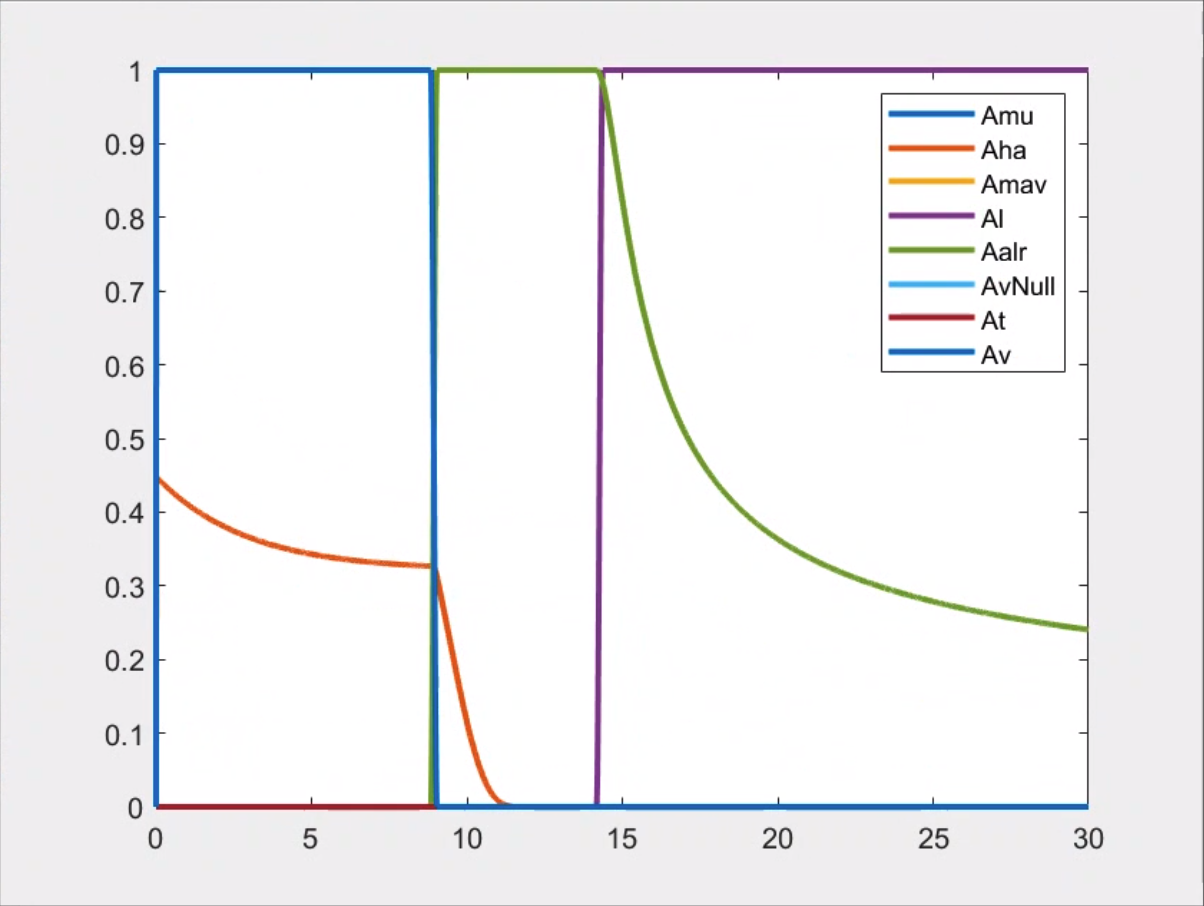
\includegraphics[width=\textwidth]{313_m_Activation.png}
\caption{Activations with medium gain}\label{act_w_m} 
\end{minipage} 
\hspace{0.2\textwidth} 
\begin{minipage}{0.40\textwidth}  
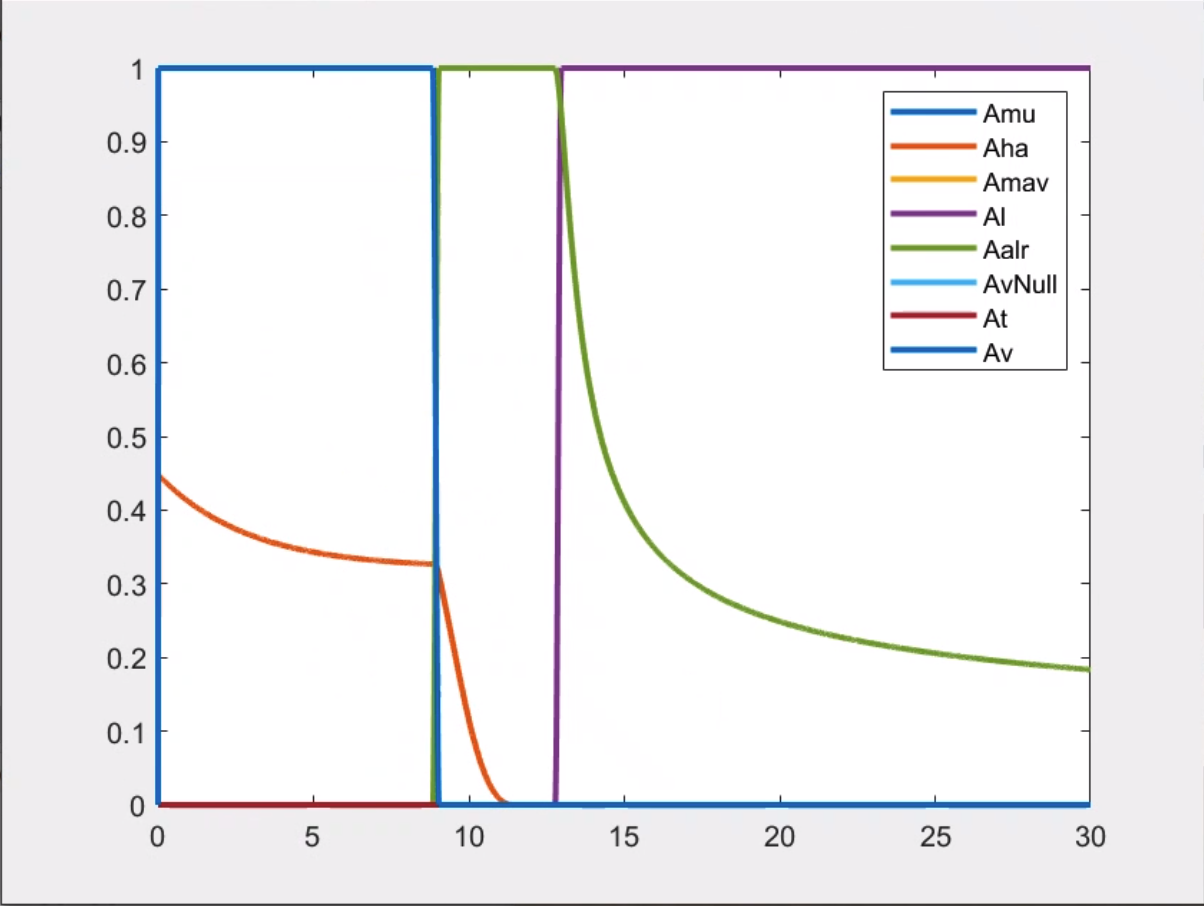
\includegraphics[width=\textwidth]{313_b_Activation.png}
\caption{Activations with big gain}\label{act_w_b} 
\end{minipage}
\end{figure}
%%%%%%%% MINI PAGE IMAGES %%%%%%%%
\begin{figure}[htpb] 
\begin{minipage}{0.40\textwidth}  
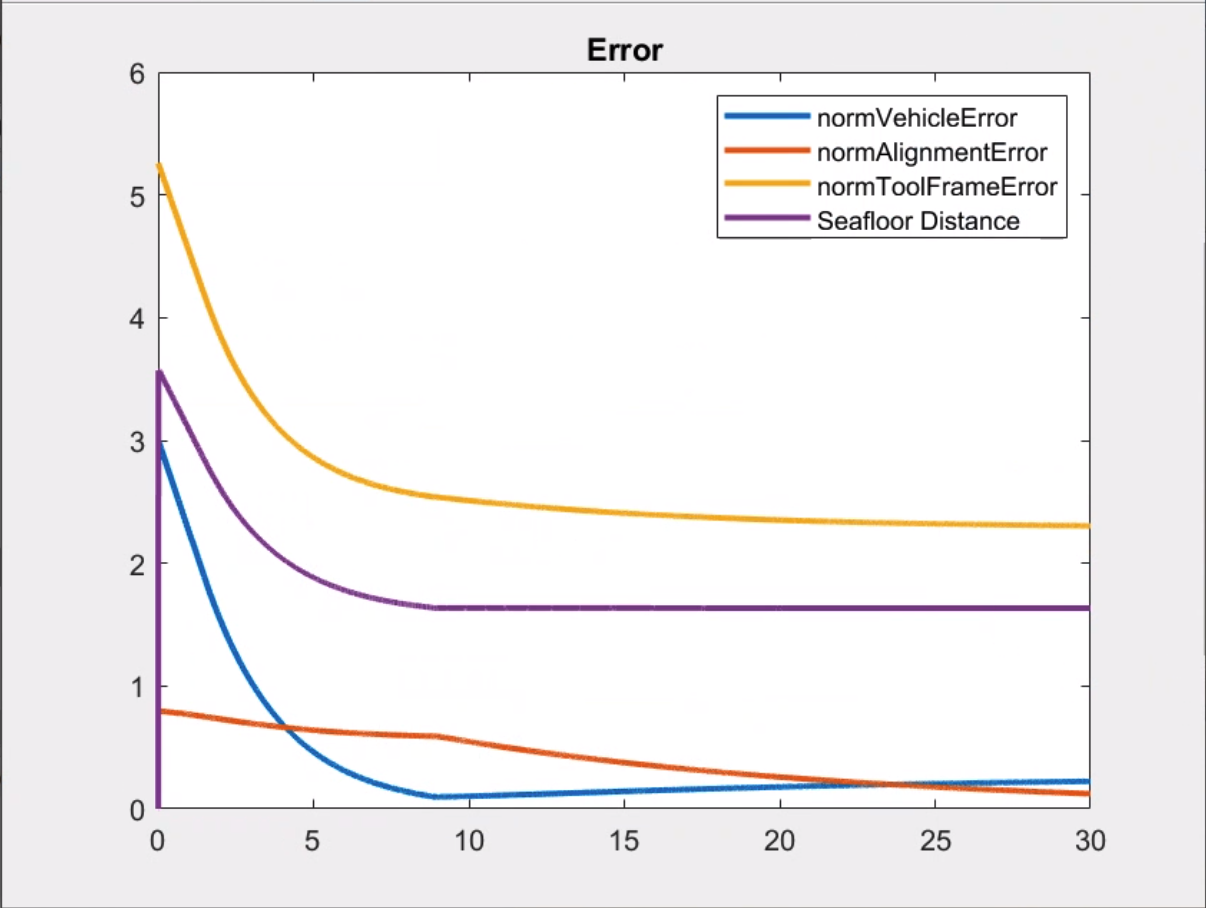
\includegraphics[width=\textwidth]{313_s_Errors.png}
\caption{Errors with small}\label{err_w_s} 
\end{minipage}  
\hspace{0.2\textwidth} 
\begin{minipage}{0.40\textwidth}  
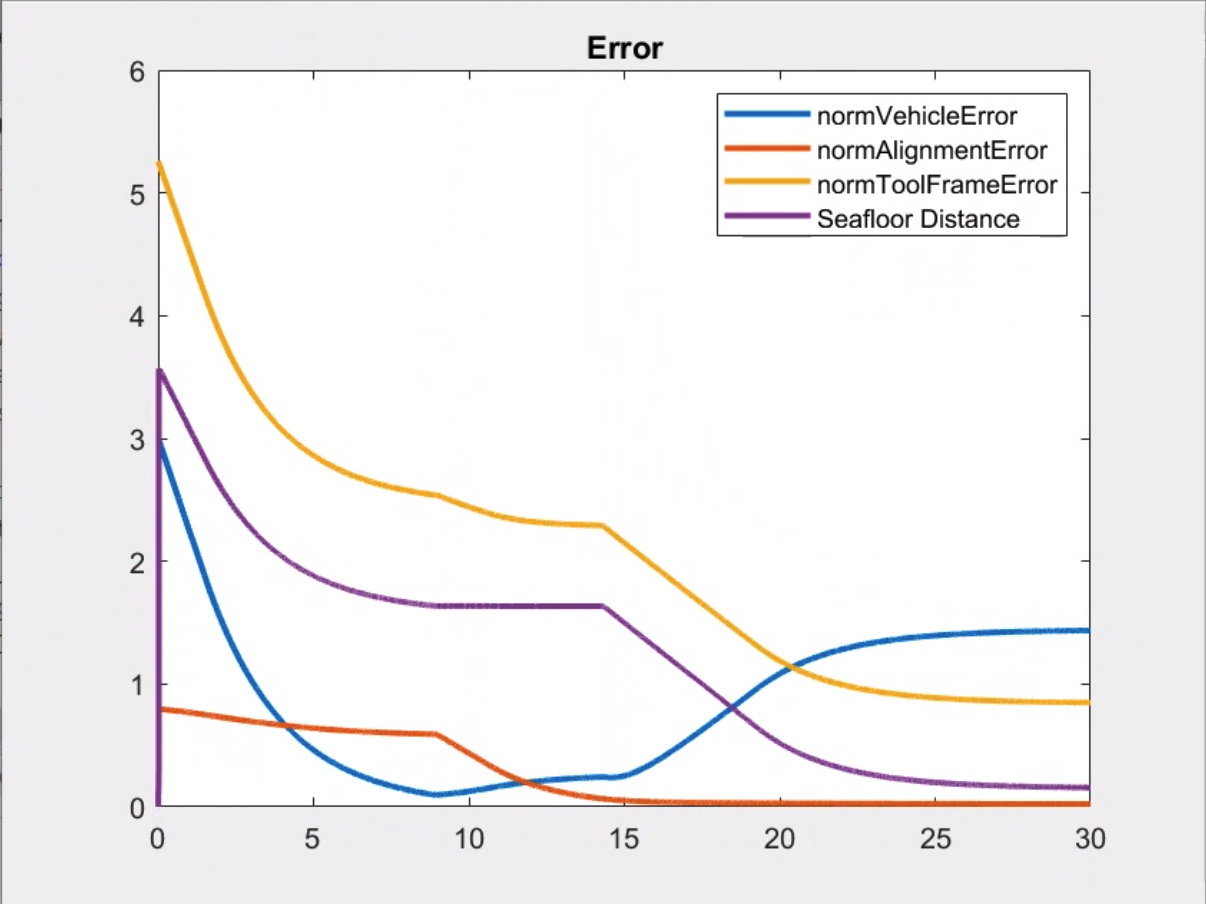
\includegraphics[width=\textwidth]{313_m_Errors.png}
\caption{Errors with medium}\label{err_w_m} 
\end{minipage} 
\hspace{0.2\textwidth} 
\begin{minipage}{0.40\textwidth}  
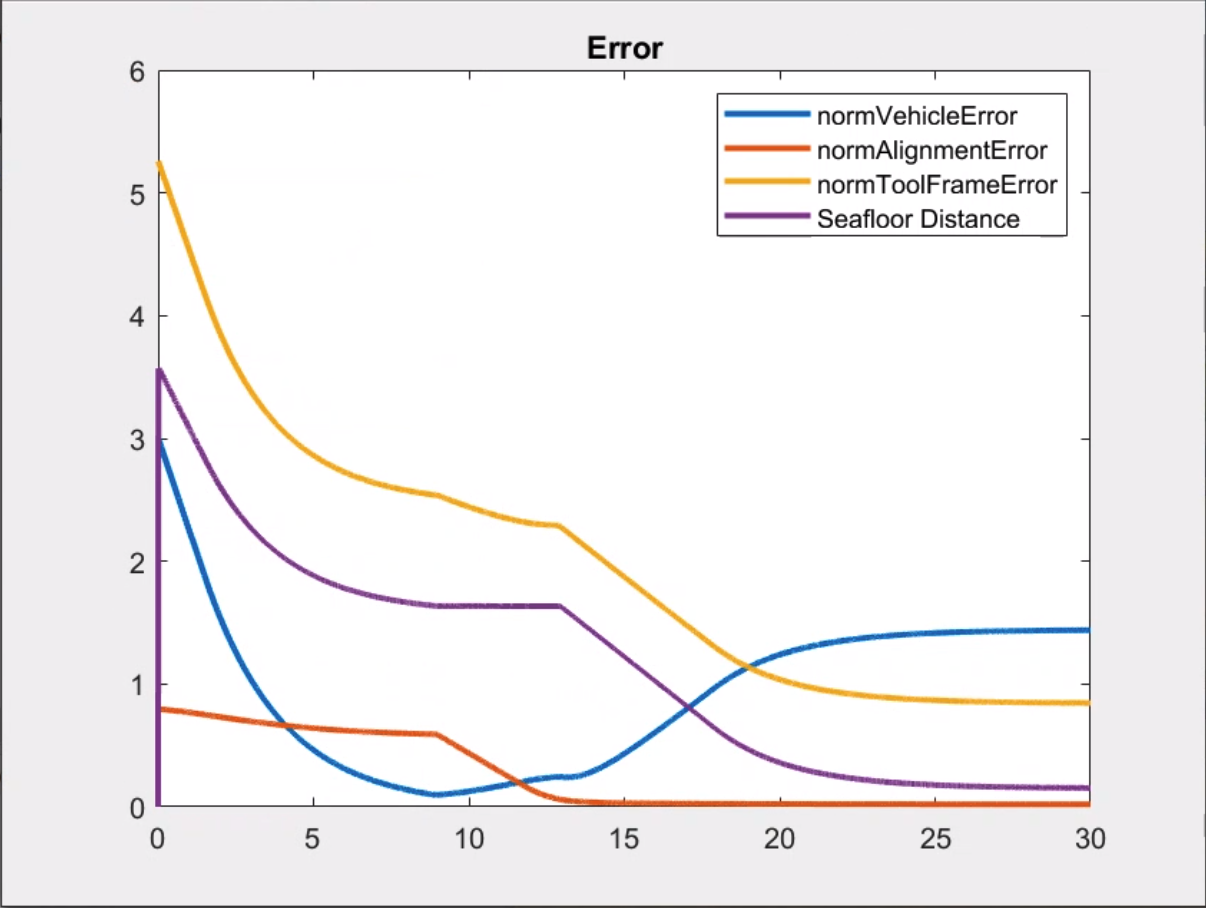
\includegraphics[width=\textwidth]{313_b_Errors.png}
\caption{Errors with big}\label{err_w_b} 
\end{minipage}
\end{figure}
%%%%%%%% MINI PAGE IMAGES %%%%%%%%

\clearpage 
\subsubsection{Q4: After the landing is accomplished, what happens if you try to move the end-effector? Is the distance to the nodule sufficient to reach it with the end-effector? Comment the observed behaviour.}\label{ex3}
The tool could reach the center of the nodule, however, we notice that the vehicle moves to help the arm to achieve the desired position. It is clear that, to avoid this problem, we need to perform a non-reactive task to constraint the vehicle not move, as we will do in the next exercise \ref{subsec:non-react}. 

\begin{figure}[h]
    \centering
    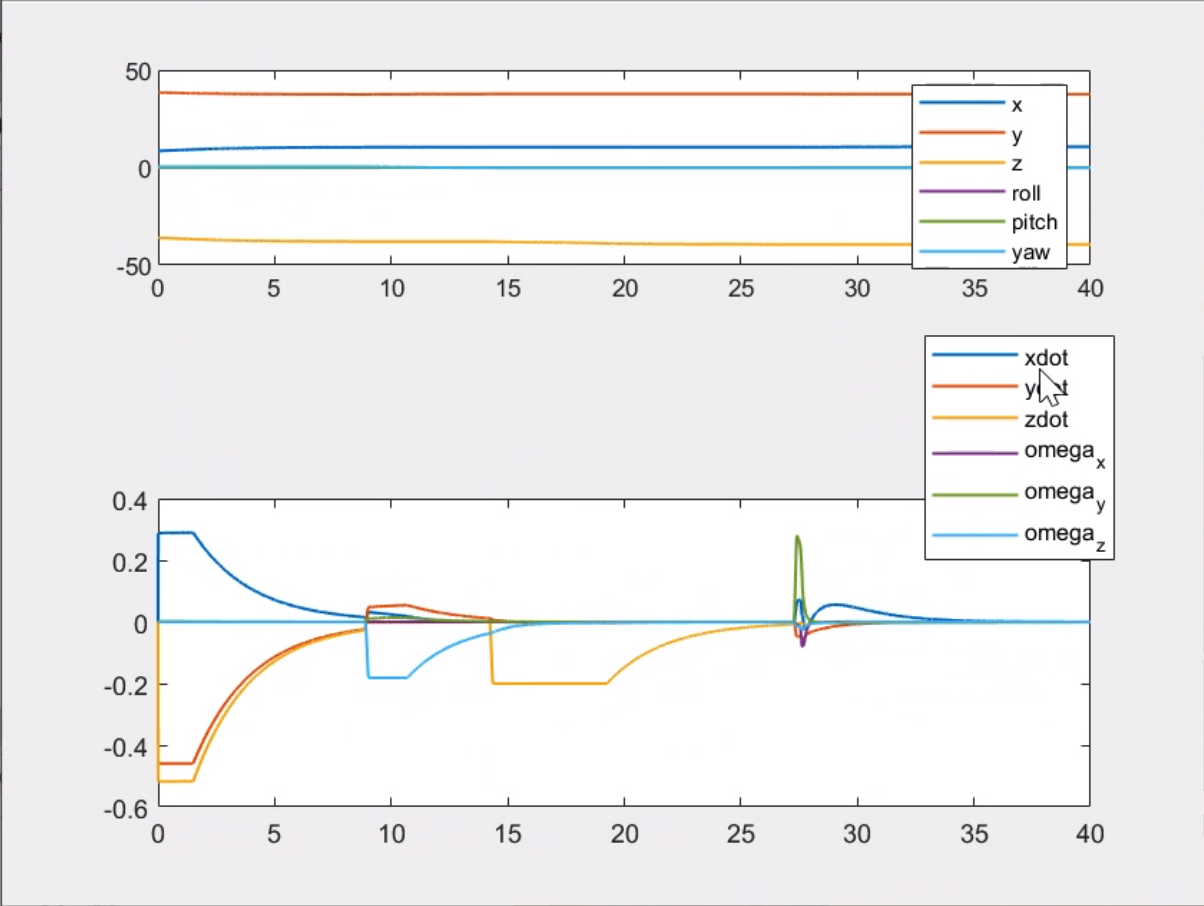
\includegraphics[scale=0.4]{314_ppdot.png}
    \caption{Visible that when tool starts move, vehicle helps it}
    \label{graphes3}
\end{figure}

\clearpage
\section{Exercise 4: Implementing a Fixed-base Manipulation Action}
\subsection{Adding non-reactive tasks} \label{subsec:non-react}
To manipulate as a fixed based manipulator, we need to constraint the vehicle to not move, otherwise the tool frame position task will make the vehicle move.

Goal: Add a constraint task that fixes the vehicle velocity to zero. Land on the seafloor. Try reaching the rock position with the end-effector, and observe that the vehicle does not move.

\subsubsection{Q1: Report the unified hierarchy of tasks used and their priorities. At which priority level did you add the constraint task?}
We have four different actions, with this hierarchy and activations:
%%%%%% TABLE %%%%%%%%%
\begin{center}
\begin{tabular}{ | c | c | c | c | c | c |}
\hline
 Control Task & \texttt{Code name} & Action A & Action B & Action C & Action D\\
 \hline
 Vehicle Null Velocity & \texttt{vNull} & Inactive & Inactive & Inactive & Active\\
 Minimum Altitude Vehicle &  \texttt{mav} & Active & Active & Inactive & Inactive \\  
 Manipulabity &  \texttt{mu} & Active & Active & Active & Active  \\
 Horizontal Attitude &  \texttt{ha} & Active & Active & Active & Active\\
 Alignment to the rock & \texttt{alr} & Inactive & Active & Active & Inactive \\
 Landing & \texttt{l} &Inactive & Inactive & Active & Inactive\\
 Tool  &  \texttt{t} & Inactive & Inactive & Inactive & Active\\
 Vehicle Position &  \texttt{v} &Active & Inactive & Inactive & Inactive\\
 \hline
\end{tabular}
\end{center}
%%%%%% TABLE %%%%%%%%%
\begin{description}
\item \textbf{Vehicle Null Velocity} [NR, E, C], it is a prerequisite task, so it has higher priority than the Action Defining tasks. Optimizazion.  \doubt
\item \textbf{Tool} [R, E, AD], it is an Action Definition task, that enable the arm to reach the tool target position. 
\end{description}

\begin{description}
	\item Action A, safe waypoint navigation with all the safety task activated
	\item Action B, alignment to the nodule with all the safety task activated
	\item Action C, landing and final rotation to be aligned with the rock
	\item Action D, now it is. performed the new Vehicle Null Velocity task, that disable the UVMS' motors, to prevent movement. The only movement will be the extension of the arm to reach the desired target tool position. 
\end{description}

%%%%%%% near images %%%%%%% 
\begin{figure}[htp]
\centering
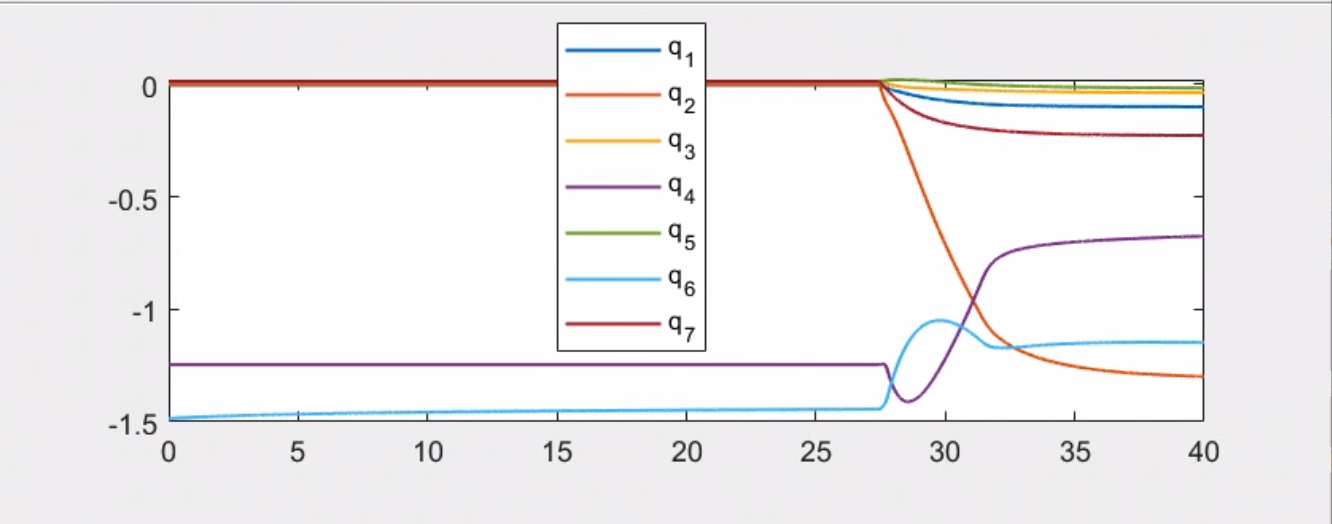
\includegraphics[width=.6\textwidth]{411_q.png}\caption{Arm joints start moving when reached task 4}
\centering
\label{fig:411_arm}
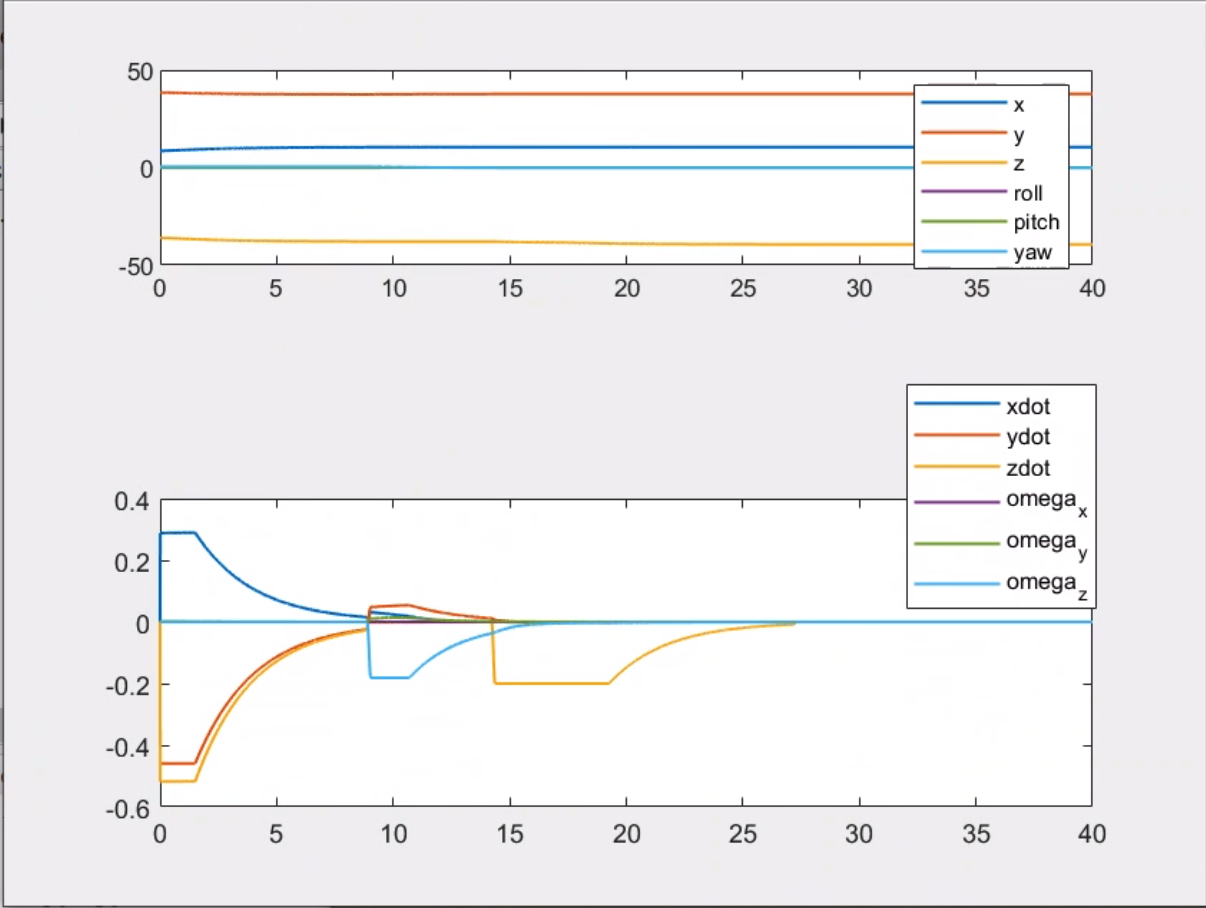
\includegraphics[width=.6\textwidth]{411_ppdot.png}\caption{Vehicle has zero velocities when task 3 is finished}
\label{fig:411_vehicle}
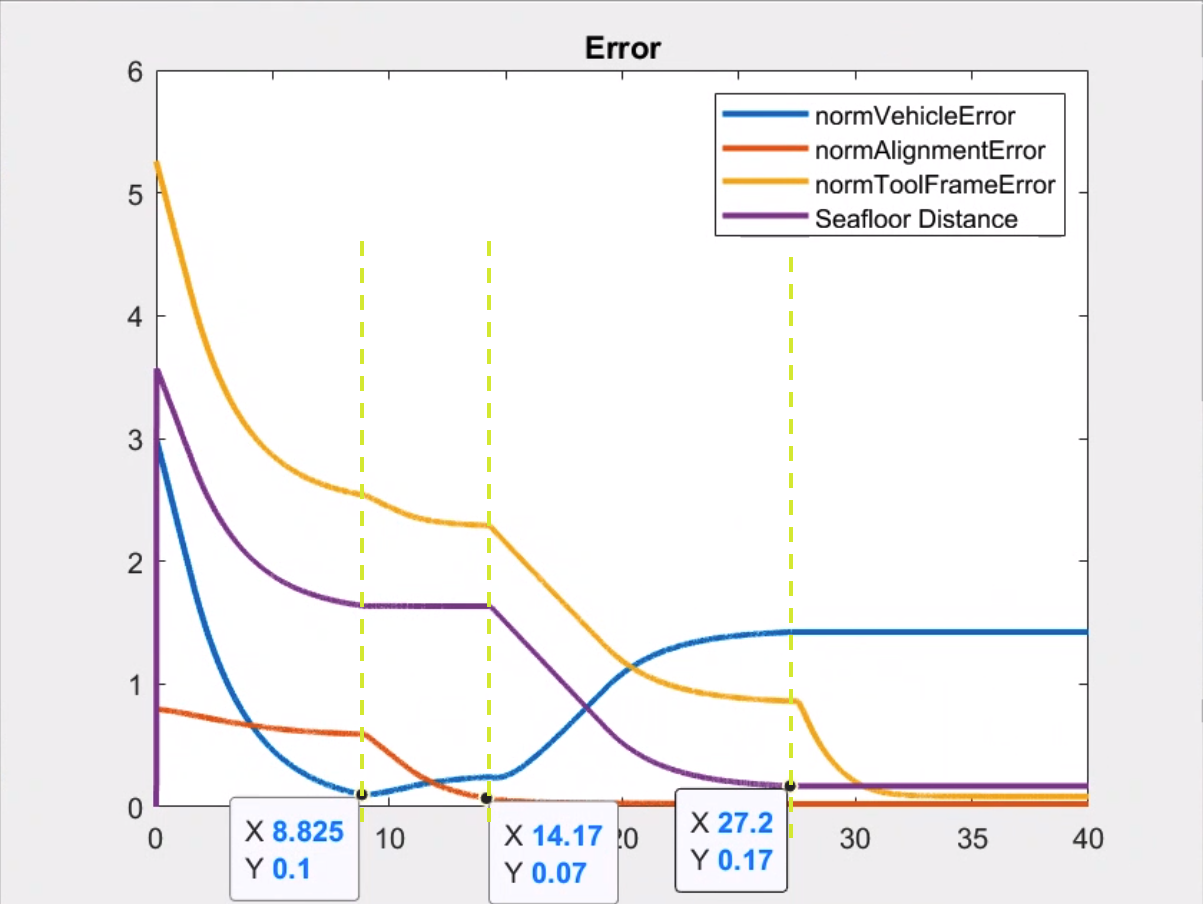
\includegraphics[width=.6\textwidth]{411_Errors.png}\caption{Vehicle has zero velocities when task 3 is finished}
\label{fig:411_errors}
\end{figure}
%%%%%%% %%%%%%%%%% %%%%%%%
\subsubsection{Q2: What is the Jacobian relationship for the Vehicle Null Velocity task? How was the task reference computed?}
The Jacobian for the Vehicle Null Velocity task is the same of the Vehicle Position, but this time we need to fix the velocity of the UVMS to zero, so we premultiply it for the zeros vector. % CI VA IL TRASPOSTO? BE SURE DI OGNI MATRIX COME é FATTA

%%%%%%% Jacobian Matrix %%%%%%% 
\begin{equation}
\boldsymbol{J}_{vehNull}=\begin{bmatrix} 0 & 0 & 0 & 0 & 0 & 0
\end{bmatrix}
    \begin{bmatrix}
     & \underset{3\times 3}{\boldsymbol{0}} & \underset{ 3\times 3}{^{w}\boldsymbol{R}_{v}} \\
     \underset{6\times 7}{\boldsymbol{0}} \\
     & \underset{ 3\times 3}{^{w}\boldsymbol{R}_{v}} & \underset{3\times 3}{\boldsymbol{0}} \\
    \end{bmatrix}
\end{equation}
%%%%%%% %%%%%%% %%%%%%% %%%%%%% 

The velocity will not change during the activation of this task because it is a Non-Reactive.

\subsubsection{Q3: Suppose the vehicle floating, i.e. not landed on the seafloor. What would happen, if due to currents, the vehicle moves?}
The Vehicle Null task cannot take in position the UVMS, it doesn't take into account disturbances, it only put velocities to zero, so it is not able to "contrastare" the current. \ocio In this scenario, the robot will start follow the current and it will go to a wrong position. The arm will continue to try to reach the desired position, but in the previous exercise \ref{ex3} the vehicle could help the arm to be able to arrive to the target, now the zero velocity has higher priority, so the vehicle could not help. 
\clearpage

\subsection{Adding a joint limit task}
Let us now constrain the arm with the actual joint limits. The vector variables \texttt{uvms.jlmin} and \texttt{uvms.jlmax} contain the maximum and minimum values respectively.

Goal: Add a joint limits avoidance task. Land on the seafloor. Try reaching the rock position with the end-effector, and observe that the vehicle does not move and that all the joints are within their limits.

\subsubsection{Q1: Report the unified hierarchy of tasks used and their priorities. At which priority level did you add the constraint task?}
We have four different actions, with this hierarchy and activations:
%%%%%% TABLE %%%%%%%%%
\begin{center}
\begin{tabular}{ | c | c | c | c | c | c |}
\hline
 Control Task & \texttt{Code name} & Action A & Action B & Action C & Action D\\
 \hline
 Vehicle Null Velocity & \texttt{vNull} & Inactive & Inactive & Inactive & Active\\
 Joint Limit & \texttt{jl} & Active & Active & Active & Active \\
 Minimum Altitude Vehicle &  \texttt{mav} & Active & Active & Inactive & Inactive \\  
 Manipulabity &  \texttt{mu} & Active & Active & Active & Active  \\
 Horizontal Attitude &  \texttt{ha} & Active & Active & Active & Active\\
 Alignment to the rock & \texttt{alr} & Inactive & Active & Active & Inactive \\
 Landing & \texttt{l} &Inactive & Inactive & Active & Inactive\\
 Tool  &  \texttt{t} & Inactive & Inactive & Inactive & Active\\
 Vehicle Position &  \texttt{v} &Active & Inactive & Inactive & Inactive\\
 \hline
\end{tabular}
\end{center}
%%%%%% TABLE %%%%%%%%%

\begin{description}
\item \textbf{Joint Limit} [R, I, S], it is a safety task, so it has higher priority than the other Action Defining tasks. It is able to control that the joints don't operate over their prefixed threshold. \ocio
\end{description}

The actions are the same as before, the only difference is that Joint Limit is always active because it is a safety task. However, it is useful when the robot perform the final action. 

\subsubsection{Q2: What is the Jacobian relationship for the Joint Limits task? How was the task reference computed?}
The Jacobian for the Joint Limit task is:
%%%%%%% Jacobian Matrix %%%%%%% 
\begin{equation}
\boldsymbol{J}_{jointLimit}=
    \begin{bmatrix}
     \underset{7\times 7}{\boldsymbol{I}} & \underset{7\times6}{\boldsymbol{0}} \\
    \end{bmatrix}
\end{equation}
%%%%%%% %%%%%%% %%%%%%% %%%%%%% 
With this Jacobian we are sure that each joint apply the limit constraints only itself and not on the other ones.
\\
We compute the \textbf{task reference} as:

%%%%%
	%\begin{center}
	%	\large
	%	$\boldsymbol{J}_{jLimits} =
	%	\begin{bmatrix}
	%	\underset{7\times7}{\boldsymbol{I}} & \underset{7\times6}{\boldsymbol{0}}
	%	\end{bmatrix}$
	%\end{center}
	%Seen that each joint influences obviously only itself for the joint limit task.\\
	
	\vspace{5px}
	\begin{equation}
		\dot{\bar{x}}_{jointLimit,i} = k
		\begin{equation}
		x_{activationMin,i} - x_{q,i},& \text{if } x_{q,i}\leq mid_i\\
		x_{activationMax,i} - x_{q,i},& \text{if } x_{q,i} > mid_i
		\end{equation}	
	\end{equation}
		%$\dot{\bar{\boldsymbol{x}}}_{jointLimit} = \begin{bmatrix} {\dot{\bar{x}}_{jLimits,1},}&{\dots,}&{\dot{\bar{x}}_{jLimits,7}} \end{bmatrix}^T $\\
		%\vspace{10px}
		% $
	where:
	\begin{description}
		\item $i = 1,\dots,7$ is the $i$-th joint.
		\item $x_{q,i}$ is the $i$ joint position ($q$)
		\item $ActivationMin$ and $ActivationMax$ are the $10\%$ of the limit imposed for each joint.
		\item $mid_i = \dfrac{x_{activationMin,i} + x_{activationMax,i}}{2}\; $ is the middle point between the Minimum Activation and the Maximum.
		\item $k$ is the gain
	\end{description}
	We use the Min and Max in order to be able to activate the joint limit when the joint arrives near the minimum guard ($ActivationMin$) or near the maximum ones ($ActivationMax$).
%%%%%%%%%
\clearpage
\section{Exercise 5: Floating Manipulation}
\subsection{Adding an optimization control objective}
Use the DexROV simulation for this exercise. 

The goal is to try to optimize the joint positions, if possible, to keep the first four joints in a "preferred shape", represented by the following vector
\begin{displaymath}
\begin{bmatrix}-0.0031 & 1.2586 & 0.0128 & -1.2460 \end{bmatrix}^\top
\end{displaymath}

Goal: Add an optimization objective to keep the first four joints of the manipulator in the preferred shape. Observe the behaviour with and without the task

\subsubsection{Q1: Report the unified hierarchy of tasks used and their priorities. At which priority level did you add the optimization task?}

\begin{itemize}
\item Joint Limit 
\item Manipulabity 
\item Horizontal Attitude 
\item Vehicle Position
\item Preferred Shape
\end {itemize}



\subsubsection{Q2: What is the Jacobian relationship for the Joint Preferred Shape task? How was the task reference computed?}

%%%%%%% Jacobian Matrix %%%%%%% 
\begin{equation}
\boldsymbol{J}_{vehNull}=
\begin{bmatrix}-0.0031 & 1.2586 & 0.0128 & -1.2460 \end{bmatrix}^\top
    \begin{bmatrix}
     \underset{4\times4}{\boldsymbol{I}} & \underset{4\times9}{\boldsymbol{0}} \\
    \end{bmatrix}
\end{equation}
%%%%%%% %%%%%%% %%%%%%% %%%%%%% 

\subsubsection{Q3: What is the difference between having or not having this objective?}

%%%%%%%% MINI PAGE IMAGES %%%%%%%%
\begin{figure}[htp]
    \centering
    \begin{minipage}{0.50\textwidth}
    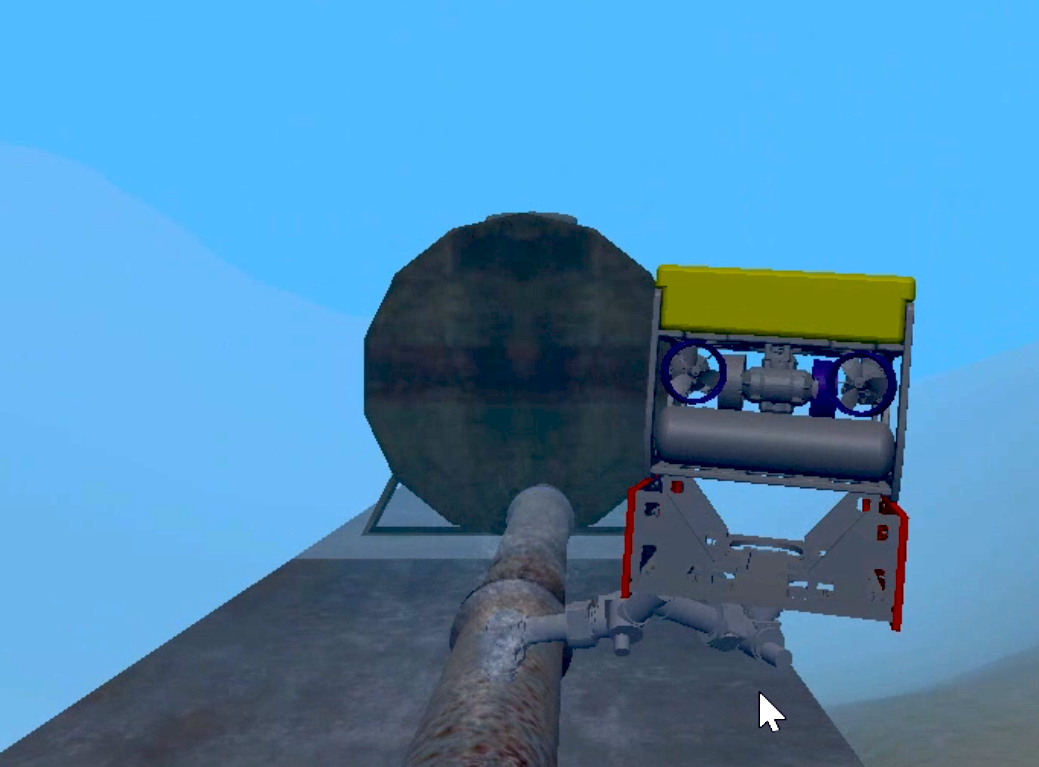
\includegraphics[scale=0.37]{513_comment.png}
    \caption{Not having}
    \end{minipage}
\hfill
    \centering
    \begin{minipage}{0.50\textwidth}
    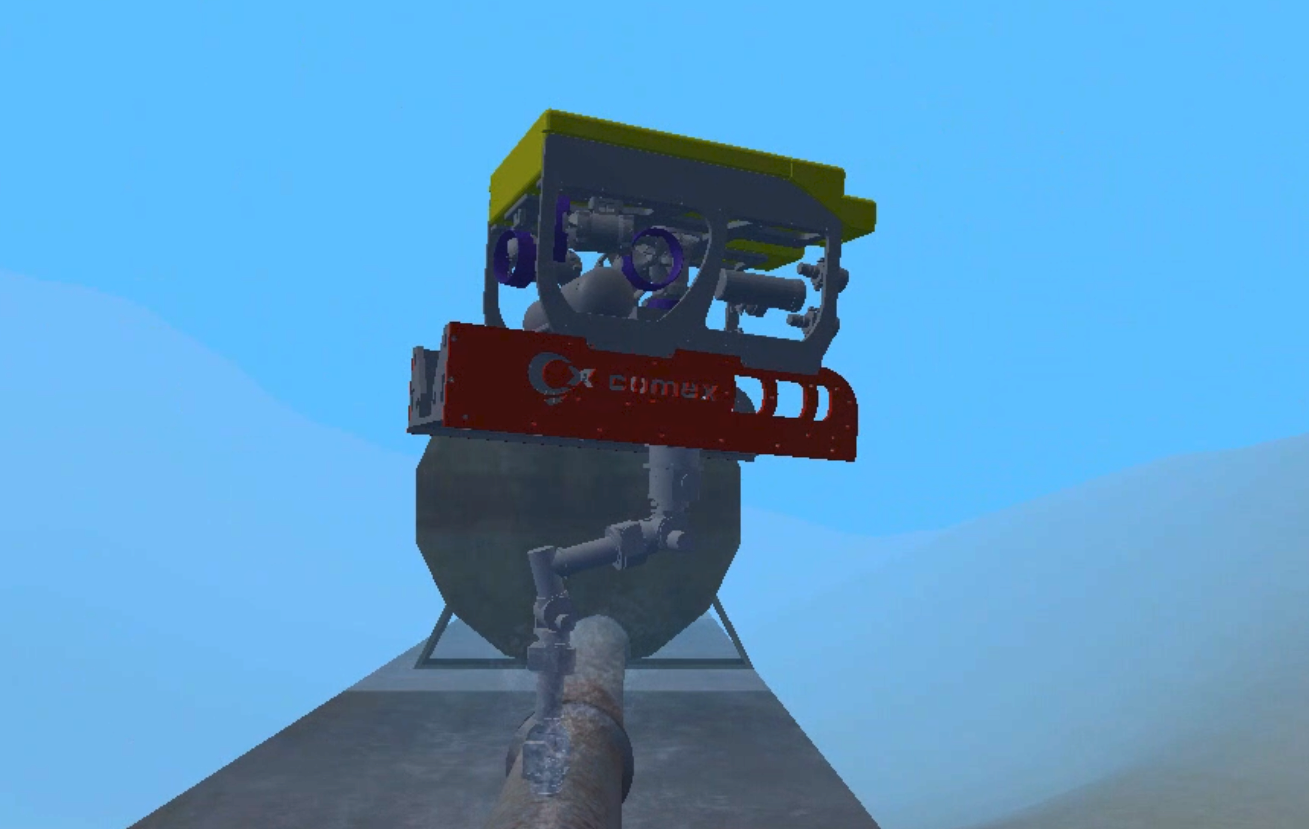
\includegraphics[scale=0.3]{513_uncomment.png}
    \caption{Having}
    \end{minipage}
\end{figure}
%%%%%%%% MINI PAGE IMAGES %%%%%%%%

\clearpage

\subsection{Adding mission phases}
Let us now structure the mission in more than one phase. In the first phase, exploit the previous exercises, and implement a safe waypoint navigation. Move the vehicle to a location close to the current defined end-effector goal position, just slightly above it. Then, trigger a change of action and perform floating manipulation.

Goal: introduce mission phases in the floating manipulation scenario. Observe the difference.

\subsubsection{Q1: Report the unified hierarchy of tasks used and their priorities. Which task is active in which phase/action?}

%%%%%% TABLE %%%%%%%%%
\begin{center}
\begin{tabular}{ | c | c | c | c |}
\hline
 Control Task & \texttt{Code name} & Action A & Action B \\
 \hline
 Vehicle Null Velocity & \texttt{vNull} & Inactive & Active \\
 Joint Limit & \texttt{jl} & Active & Active \\
 Manipulabity &  \texttt{mu} & Active & Active\\
 Horizontal Attitude &  \texttt{ha} & Active & Active \\
 Tool  &  \texttt{t} & Inactive & Active\\
 Vehicle Position &  \texttt{v} &Active & Inactive\\
 Preferred Shape & \texttt{ps} & Active & Active\\
 \hline
\end{tabular}
\end{center}
%%%%%% TABLE %%%%%%%%%

\subsubsection{Q2: What is the difference with the previous simulation (still in exercise 5), where only one action was used?}

%%%%%%%% MINI PAGE IMAGES %%%%%%%%
\begin{figure}[htpb] 
\begin{minipage}{0.40\textwidth} 
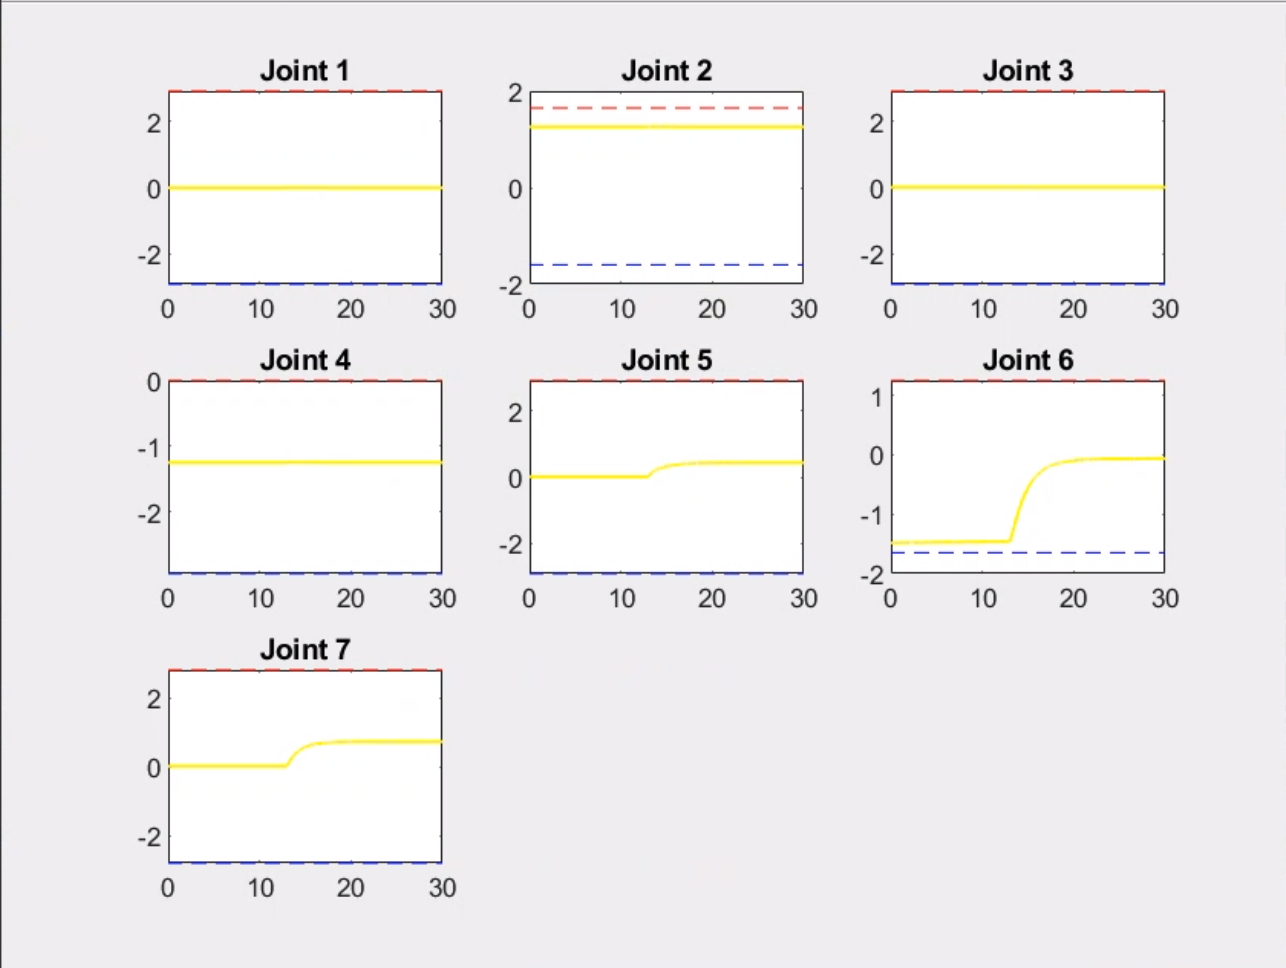
\includegraphics[width=\textwidth]{522_1_wout_TPIK2.png} 
\caption[Joint limits: without TPIK2]{Joint limits: without TPIK2}\label{JL_wout_TPIK2} 
\end{minipage} 
\hspace{0.2\textwidth} 
\begin{minipage}{0.40\textwidth}  
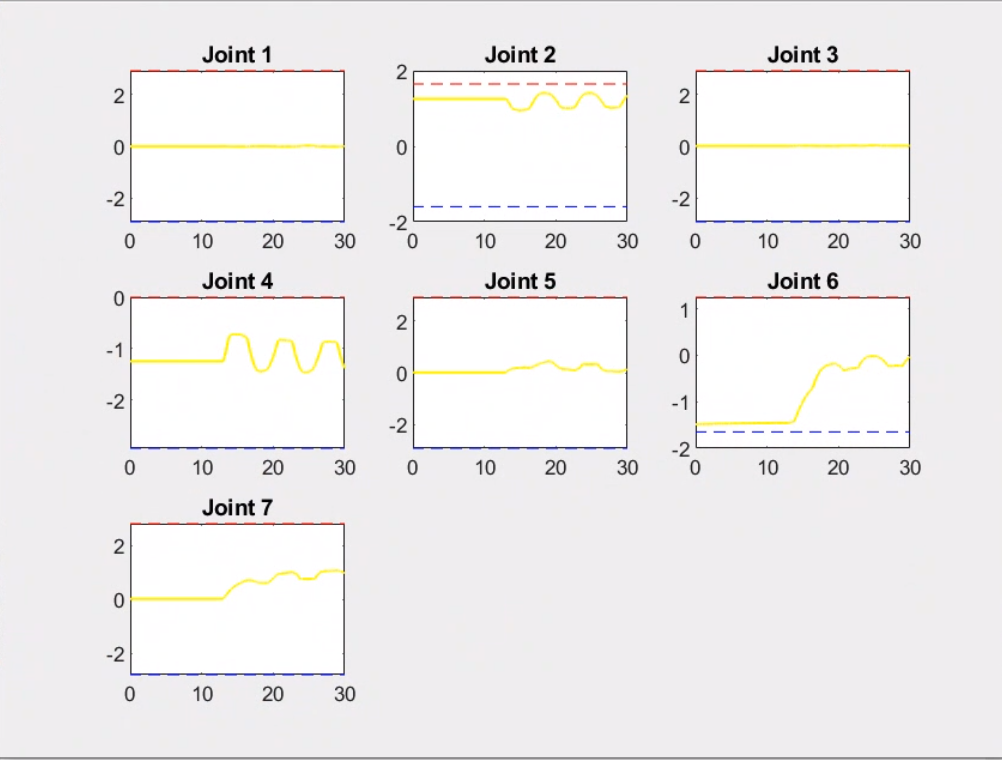
\includegraphics[width=\textwidth]{522_1_w_TPIK2.png}
\caption[Joint limits: with TPIK2]{Joint limits: with TPIK2}\label{JL_w_TPIK2} 
\end{minipage}  
\end{figure}
%%%%%%%% MINI PAGE IMAGES %%%%%%%%
\begin{figure}[htpb] 
\begin{minipage}{0.40\textwidth} 
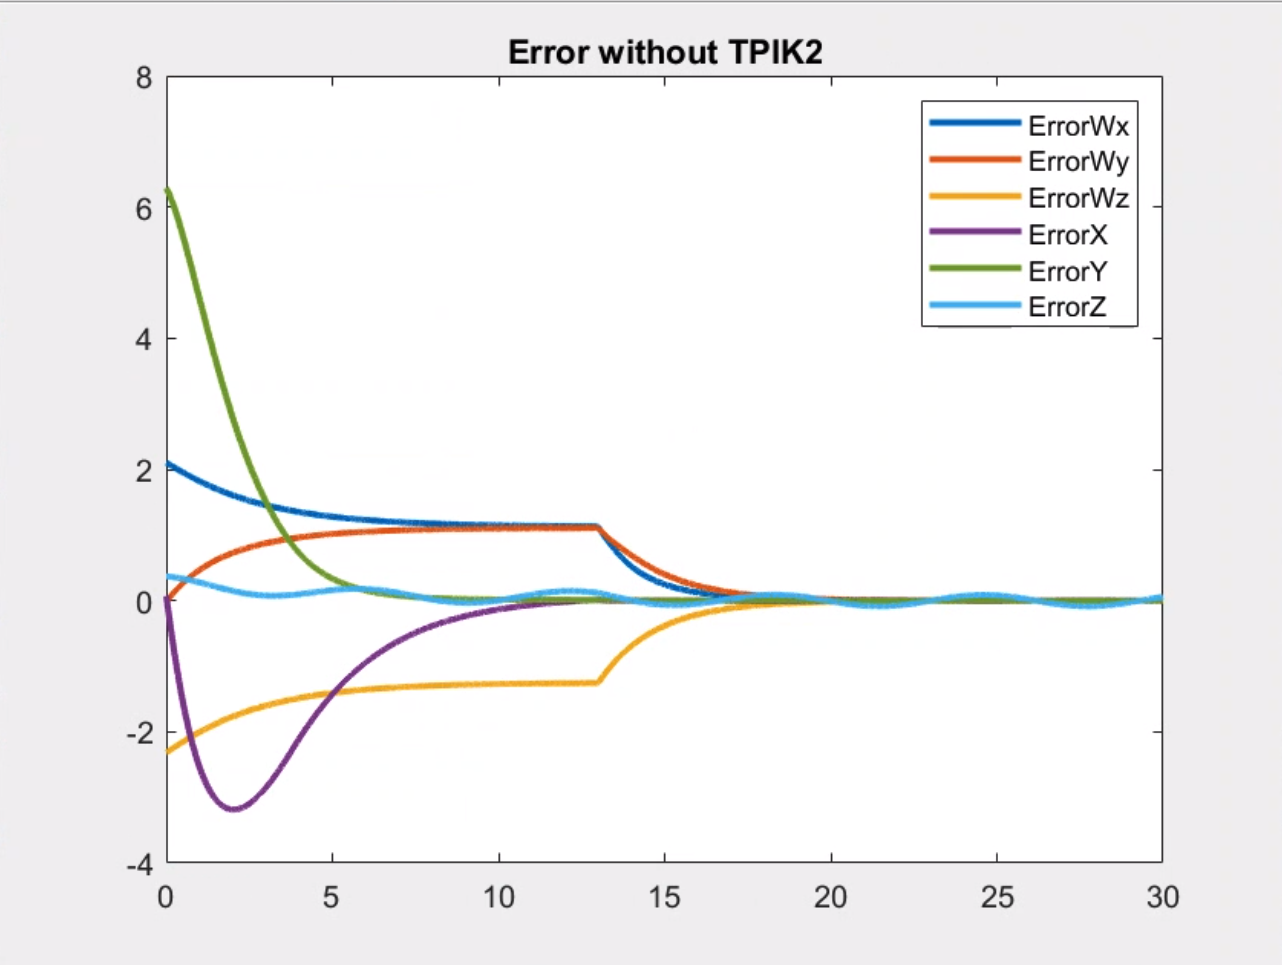
\includegraphics[width=\textwidth]{522_2_wout_TPIK2.png} 
\caption[Errors: without TPIK2]{Errors: without TPIK2}\label{Error_wout_TPIK2} 
\end{minipage} 
\hspace{0.2\textwidth} 
\begin{minipage}{0.40\textwidth}  
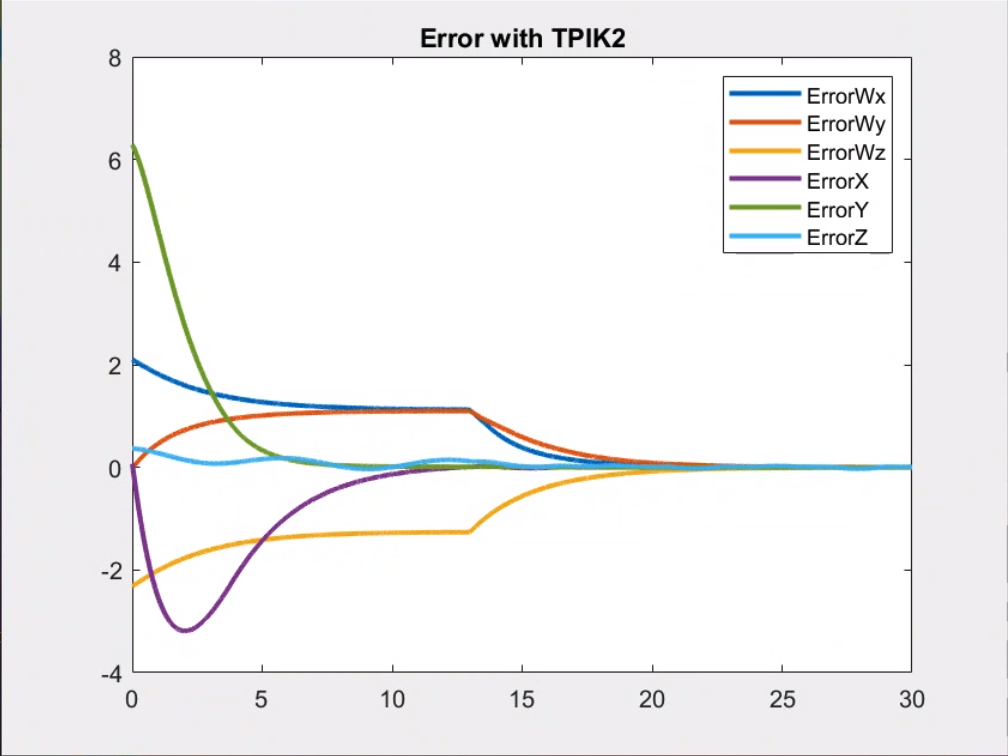
\includegraphics[width=\textwidth]{522_2_w_TPIK2.png}
\caption[Errors: with TPIK2]{Errors: with TPIK2}\label{Error_w_TPIK2} 
\end{minipage}  
\end{figure}
%%%%%%%% MINI PAGE IMAGES %%%%%%%%
\begin{figure}[htpb] 
\begin{minipage}{0.40\textwidth} 
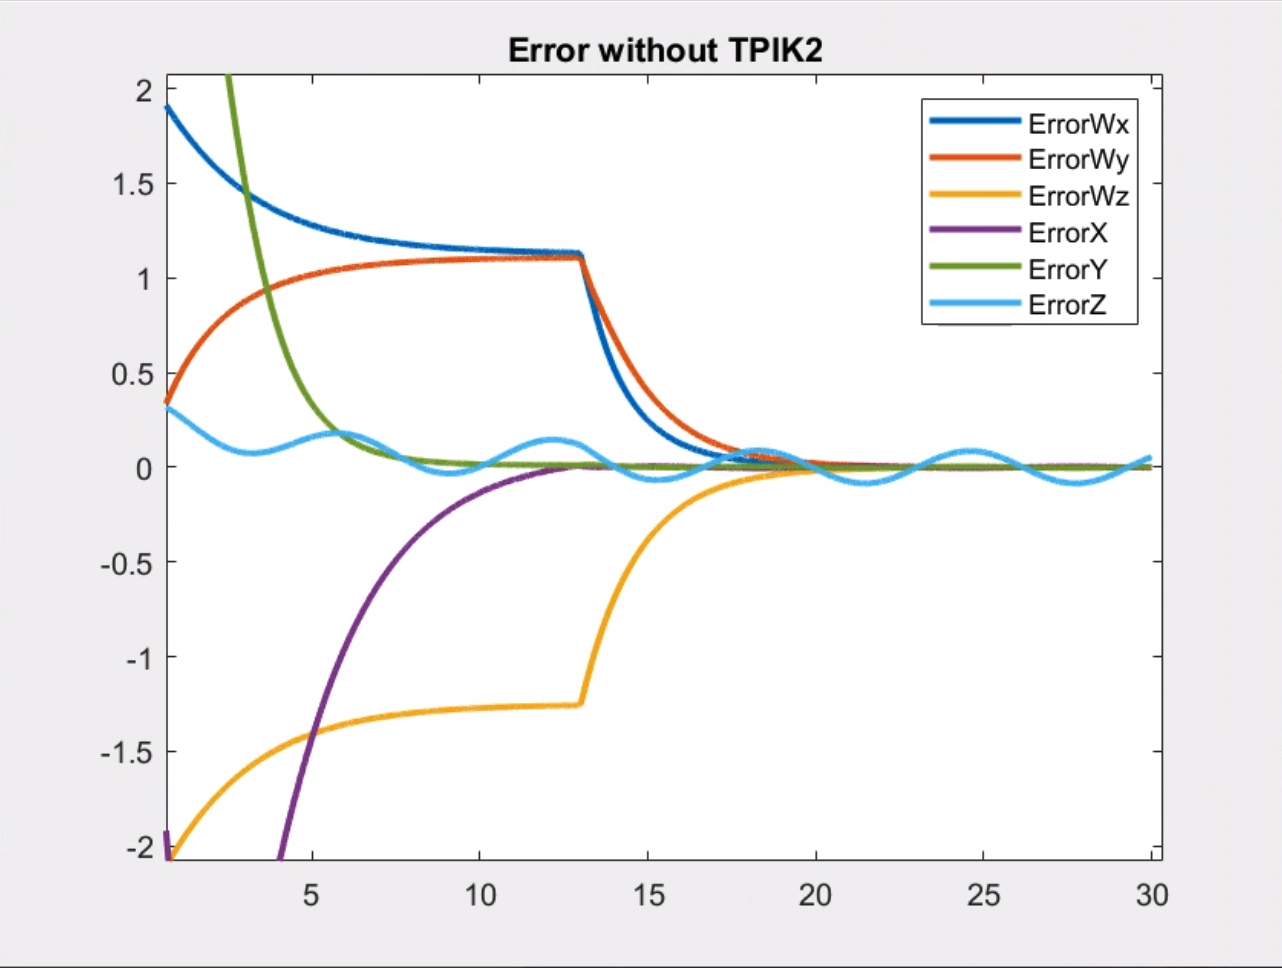
\includegraphics[width=\textwidth]{522_3_wout_TPIK2.png} 
\caption[Zoomed Error: without TPIK2]{Zoomed Error: without TPIK2}\label{zoomed_error_wout_TPIK2} 
\end{minipage} 
\hspace{0.2\textwidth} 
\begin{minipage}{0.40\textwidth}  
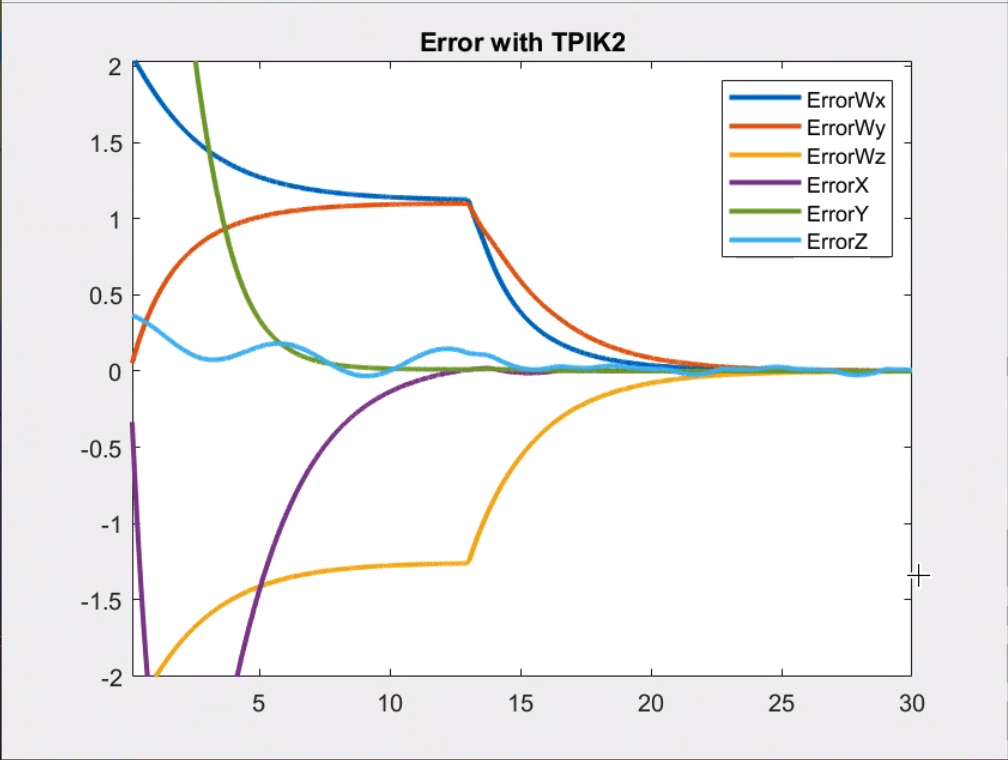
\includegraphics[width=\textwidth]{522_3_w_TPIK2.png}
\caption[Zoomed Error: with TPIK2]{Zoomed Error: with TPIK2}\label{zoomed_error_w_TPIK2} 
\end{minipage}  
\end{figure}
%%%%%%%% MINI PAGE IMAGES %%%%%%%%
\begin{figure}[htpb] 
\begin{minipage}{0.40\textwidth} 
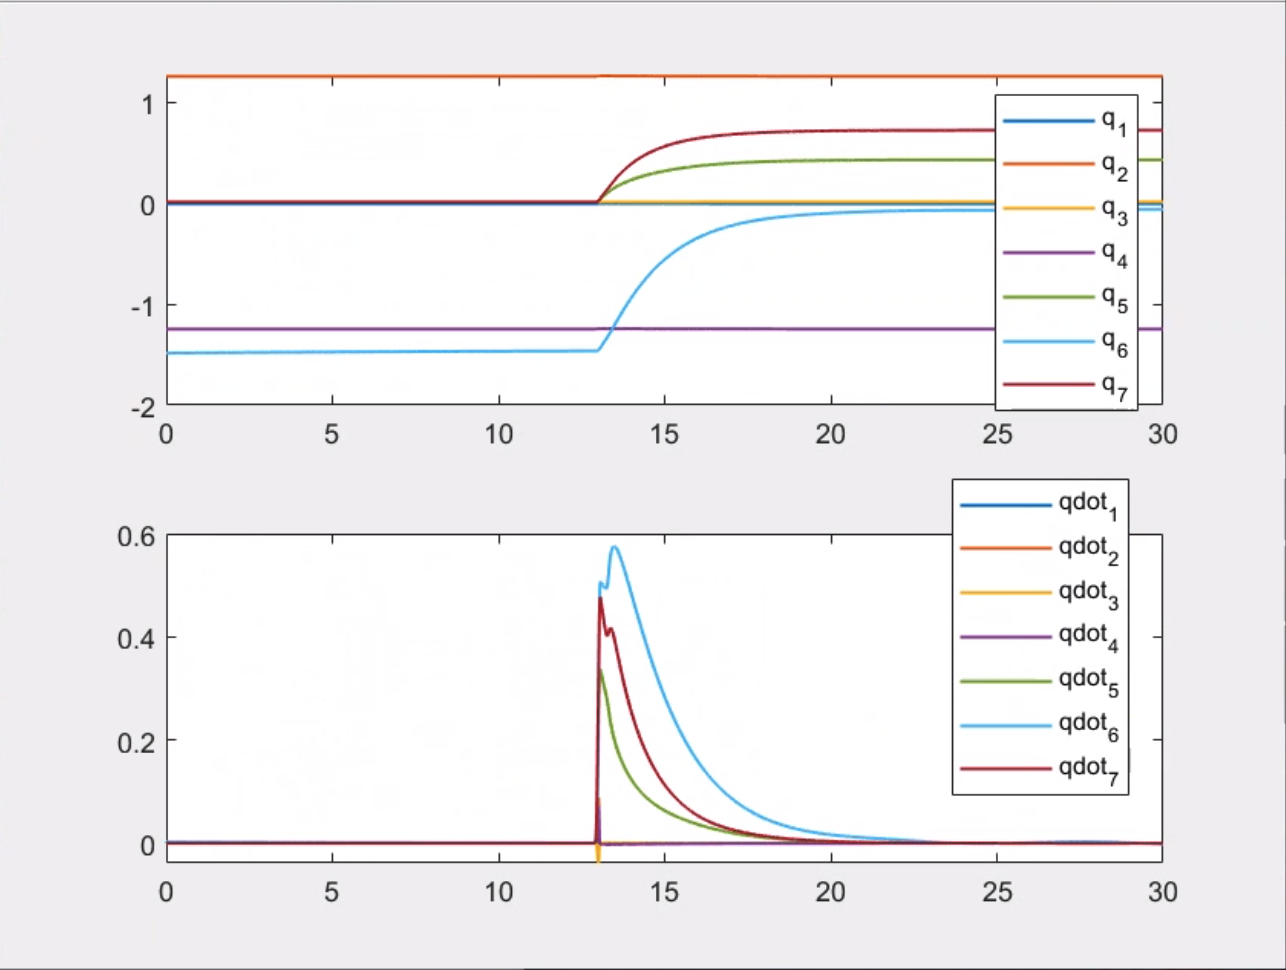
\includegraphics[width=\textwidth]{522_4_wout_TPIK2.png} 
\caption[Joints configurations and velocities: without TPIK2]{Joints configurations and velocities: without TPIK2}\label{Jqandqdot_wout_TPIK2} 
\end{minipage} 
\hspace{0.2\textwidth} 
\begin{minipage}{0.40\textwidth}  
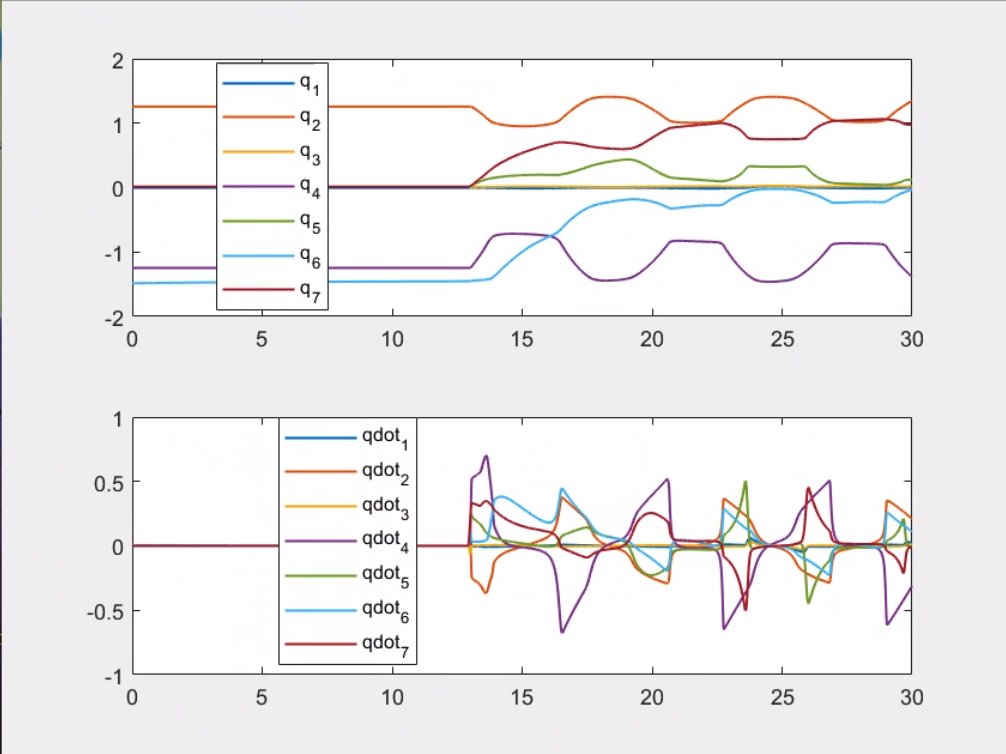
\includegraphics[width=\textwidth]{522_4_w_TPIK2.png}
\caption[Joints configurations and velocities: with TPIK2]{Joints configurations and velocities: with TPIK2}\label{Jqandqdot_w_TPIK2} 
\end{minipage}  
\end{figure}
%%%%%%%%%%%%%%%%%%%%%%%%%%%


\clearpage
\section{Exercise 6: Floating Manipulation with Arm-Vehicle Coordination Scheme}
\subsection{Adding the parallel arm-vehicle coordination scheme}
Let us now see how the two different subsystems (arm and vehicle) can be properly coordinate. Introduce in the simulation a sinusoidal velocity disturbance acting on the vehicle, and assume the actual vehicle velocity measurable. To do so, add a constant (in the inertial frame) velocity vector to the reference vehicle velocity before integrating it in the simulator. 

Goal: modify the control part to implement the parallel arm-vehicle coordination scheme. Observe that, even with a disturbance acting on the vehicle, the end-effector can stay in the required constant position.

\subsubsection{Q1: Which tasks did you introduce to implement the parallel coordination scheme?}

vConstraint - Nel TPIK2.

Non è coordinato senza il TPIK 2 , non reagisce ai cambi dovuti al 

\subsubsection{Q2: What happens if the sinusoidal disturbance becomes too big?}



%\begin{figure}[t]
%	\centering
%	\subfloat[]{\includegraphics[height=7cm]{trident.jpg}}\label{fig:trident}
%	\subfloat[]{\includegraphics[height=7cm]{maris.jpg}}\label{fig:maris}
%	\caption{(a) TRIDENT UVMS (b) MARIS UVMS.}\label{fig:uvms_examples}
%\end{figure}


		
%		\begin{figure}[b]
%			\centering
%			\subfloat[]{\frame{\includegraphics[keepaspectratio,height=3cm]{trident1.eps}}} 
%			\subfloat[]{\frame{\includegraphics[keepaspectratio,height=3cm]{trident2.eps}}}
%			\subfloat[]{\frame{\includegraphics[keepaspectratio,height=3cm]{trident3.eps}}}
%			\subfloat[]{\frame{\includegraphics[keepaspectratio,height=3cm]{trident4.eps}}}
%			\caption{Sequence of snapshots taken from the onboard camera during the TRIDENT final experiments.}
%			\label{fig_tri_trial_maiorca_img}
%		\end{figure}


\end{document}

